\documentclass[a4paper,12pt]{article}

% Paquetes básicos
\usepackage[utf8]{inputenc}
\usepackage[T1]{fontenc}
\usepackage[spanish]{babel}
\usepackage{graphicx}
\usepackage{xcolor}
\usepackage{lipsum}
\usepackage{geometry}
\geometry{top=3cm, bottom=3cm, left=2.5cm, right=2.5cm}

% Paquetes para diseño
\usepackage{titlesec}
\usepackage{fancyhdr}
\usepackage{amsmath}
\usepackage{textgreek}
\usepackage{amssymb}
\usepackage{hyperref}

% Paquetes para el entorno lstlisting
\usepackage{listings}
\usepackage{inconsolata}

%encabezado y pie de página nivel profesional
\usepackage{fancyhdr}
\pagestyle{fancy}
\fancyhf{}
\fancyhead[L]{\leftmark}
\fancyhead[R]{\rightmark}
\fancyfoot[L]{\textbf{Ismael Sallami Moreno - GIIADE}}
\fancyfoot[C]{\thepage}
\fancyfoot[R]{\textbf{(UGR)} \today}
\renewcommand{\headrulewidth}{0.4pt}
\renewcommand{\footrulewidth}{0.4pt}
\setlength{\headheight}{15pt}
\setlength{\headsep}{10pt}
\setlength{\footskip}{20pt}
\usepackage{truncate}
\fancyhead[L]{\truncate{0.5\headwidth}{\leftmark}}
\fancyhead[R]{\truncate{0.5\headwidth}{\rightmark}}
\usepackage{mathpazo}
\usepackage{tcolorbox}
\usepackage{array}
\usepackage{csquotes}



% Paquete para fondo
\usepackage{background}
\usepackage{float}

% Configuración de lstlisting
\lstset{
    inputencoding=utf8,          % Permite UTF-8
    extendedchars=true,          % Reconoce caracteres extendidos
    literate=                    % Configuración manual para tildes y símbolos
        {á}{{\'a}}1
        {é}{{\'e}}1
        {í}{{\'i}}1
        {ó}{{\'o}}1
        {ú}{{\'u}}1
        {ñ}{{\~n}}1
        {Á}{{\'A}}1
        {É}{{\'E}}1
        {Í}{{\'I}}1
        {Ó}{{\'O}}1
        {Ú}{{\'U}}1
        {Ñ}{{\~N}}1
        {¿}{{\textquestiondown}}1
        {¡}{{\textexclamdown}}1,
    basicstyle=\ttfamily,        % Fuente monoespaciada
    breaklines=true,             % Habilita salto de línea automático
    frame=single,                % Marco alrededor del código
    backgroundcolor=\color{gray!10}, % Fondo gris claro
    keywordstyle=\color{blue},   % Color para palabras clave
    commentstyle=\color{green},  % Color para comentarios
    stringstyle=\color{red}      % Color para strings
}
\lstdefinestyle{customcpp}{
    language=C++,                % Lenguaje de programación
    showspaces=false,            % No mostrar espacios
    showtabs=false,              % No mostrar tabulaciones
    tabsize=4,                   % Tamaño de tabulación
    showstringspaces=false,      % No mostrar espacios en strings
    numbers=left,                % Números de línea a la izquierda
    numberstyle=\tiny\color{gray}, % Estilo de los números de línea
    numbersep=5pt,               % Separación de los números de línea
    stepnumber=1,                % Mostrar número en cada línea
    basicstyle=\ttfamily\footnotesize, % Estilo básico del código
    keywordstyle=\bfseries\color{blue}, % Estilo de las palabras clave
    commentstyle=\itshape\color{green!50!black}, % Estilo de los comentarios
    stringstyle=\color{red},     % Estilo de los strings
    identifierstyle=\color{black}, % Estilo de los identificadores
    % procnamekeys={def,class},    % Palabras clave para nombres de funciones
    morekeywords={constexpr,nullptr,size_t}, % Más palabras clave
    emph={int,char,double,float,unsigned}, % Palabras a enfatizar
    emphstyle=\color{magenta},   % Estilo de las palabras enfatizadas
    backgroundcolor=\color{gray!10}, % Color de fondo
    frame=shadowbox,             % Marco con sombra
    rulesepcolor=\color{gray},   % Color de la línea de separación
    breakatwhitespace=false,     % No cortar en espacios en blanco
    breaklines=true,             % Cortar líneas largas
    captionpos=b,                % Posición del título (abajo)
    escapeinside={(*@}{@*)},     % Delimitadores para escapar a LaTeX
    morecomment=[l][\color{magenta}]{\#}, % Comentarios de una línea
    morecomment=[s][\color{orange}]{/*}{*/}, % Comentarios multilínea
    morestring=[b],             % Strings entre comillas dobles
    morestring=[b]'              % Strings entre comillas simples
}

% Configuración de título
\titleformat{\section}{\normalfont\Large\bfseries}{\thesection}{1em}{}

% Información del documento
\title{
    \vspace{-2cm}
    
\includegraphics[width=0.3\textwidth]{images/etsiit.png} \\ % Cambia el logo si es necesario
    \LARGE Ingeniería Informática + ADE\\
    \large Universidad de Granada (UGR)\\[1cm]
}
\author{\textbf{Autor:} Ismael Sallami Moreno}
\date{\textbf{Asignatura:} Tema 5: Capa de Aplicación (FR)\\[1cm]}

% Configuración del fondo
\backgroundsetup{
    scale=1,
    color=black,
    opacity=0.2,
    angle=0,
    position=current page.south,
    vshift=0pt,
    hshift=0pt,
    contents={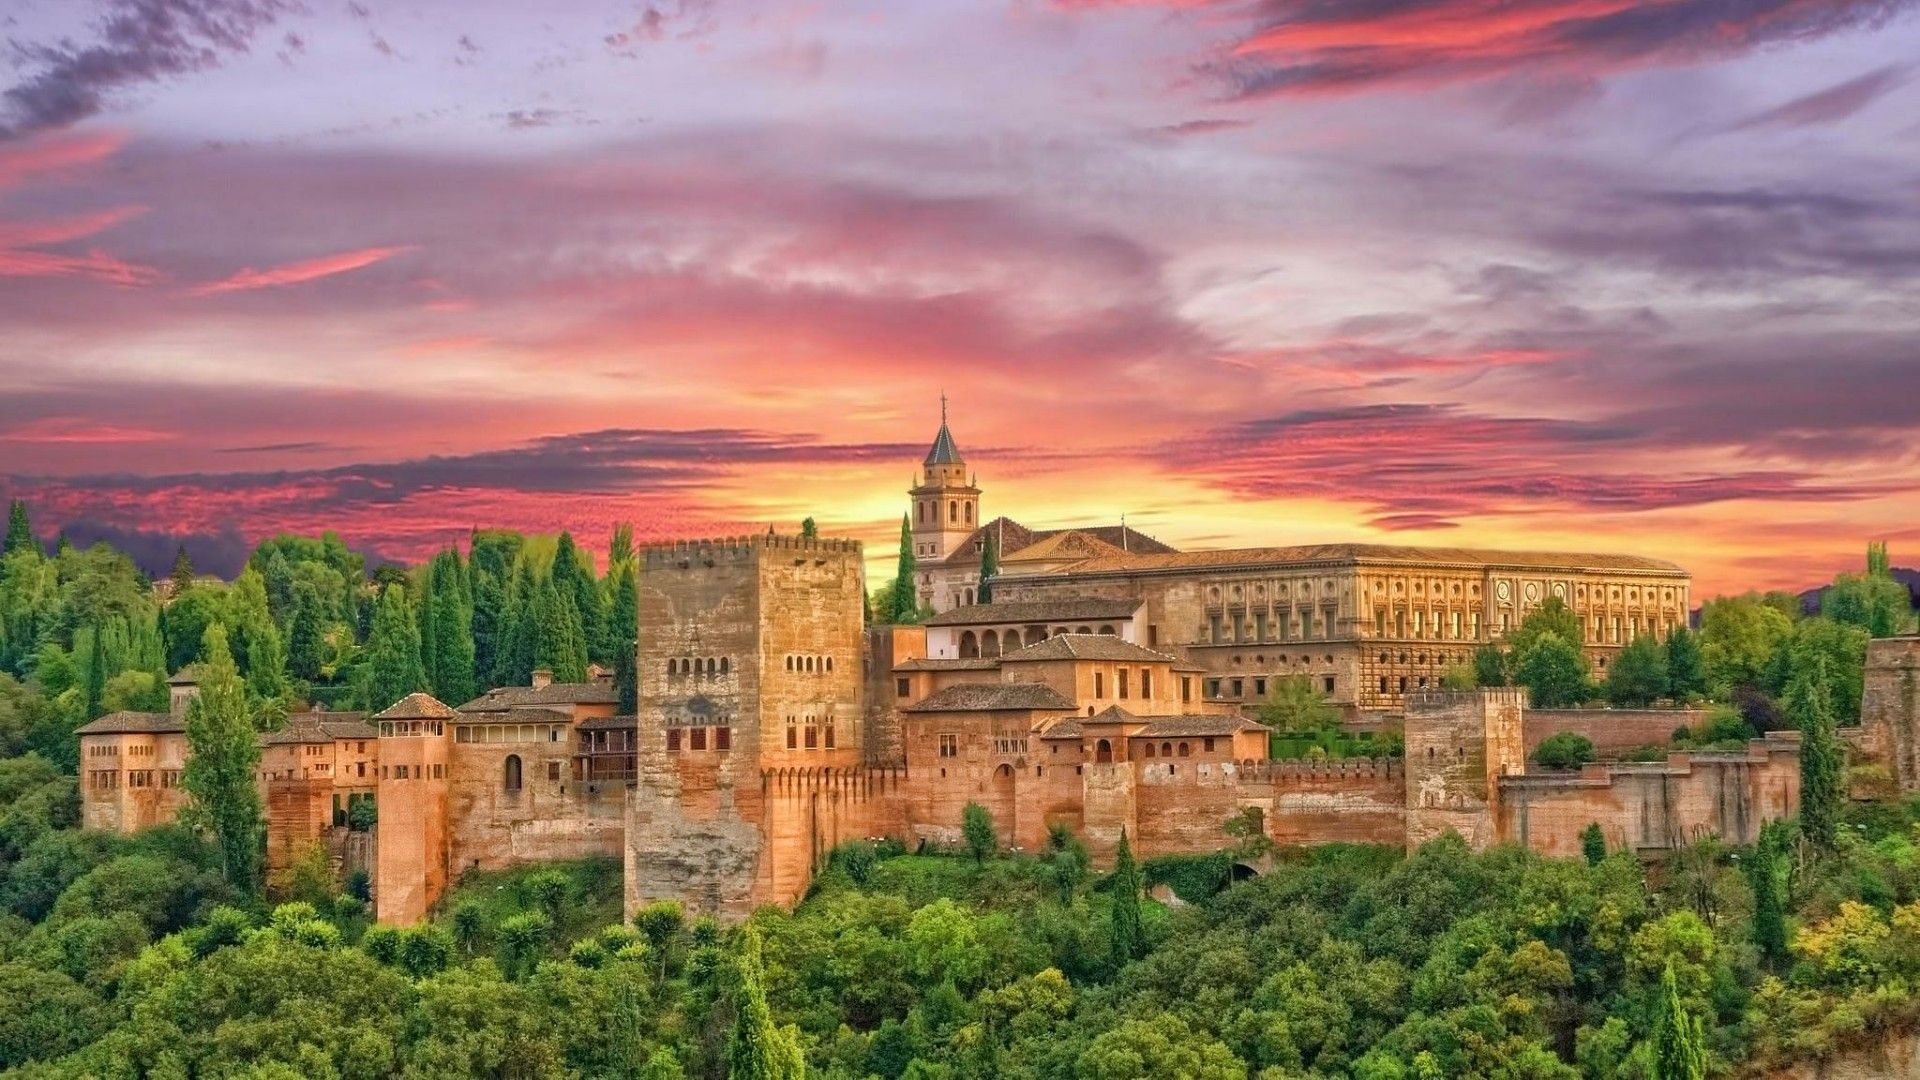
\includegraphics[width=\paperwidth,height=\paperheight,keepaspectratio]{images/granada.jpg}}
}

% Inicio del documento
\begin{document}

% Portada
\maketitle
\thispagestyle{empty}

\begin{center}
    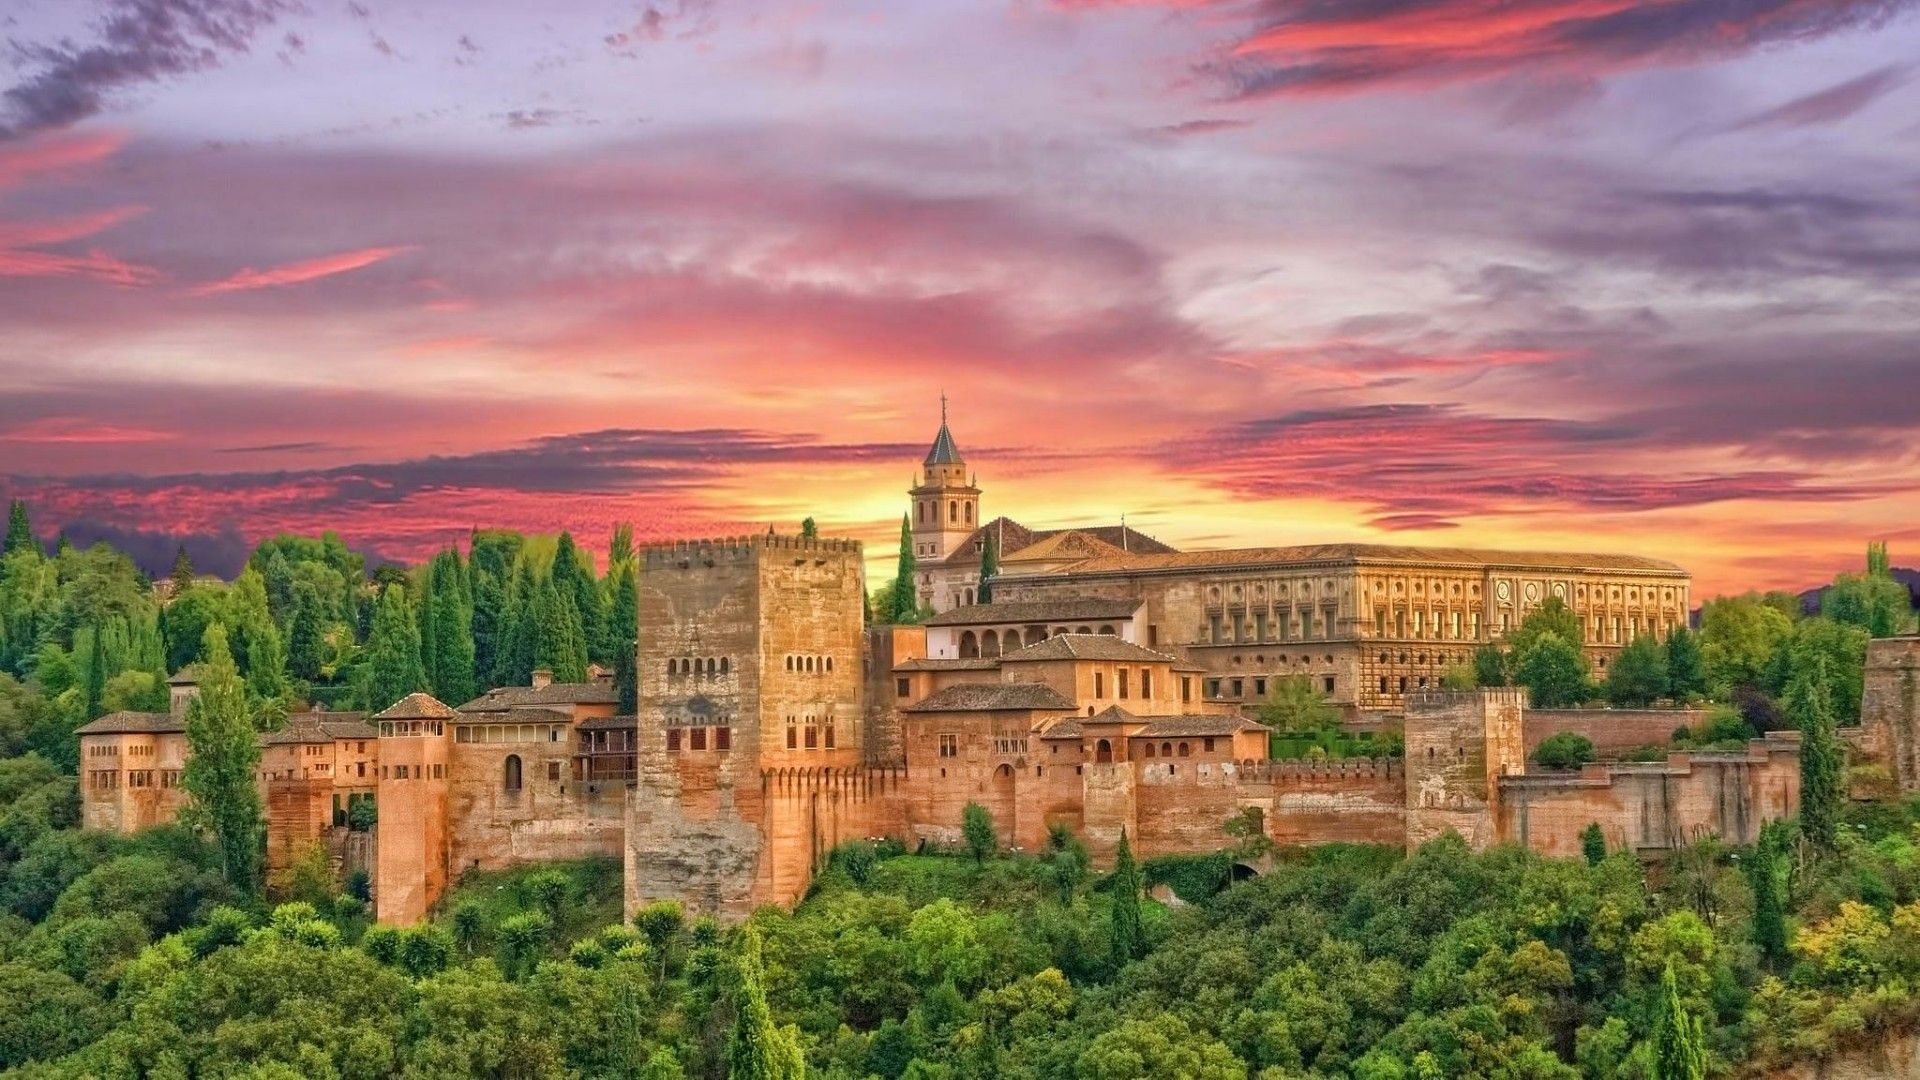
\includegraphics[width=\textwidth,height=0.4\textheight,keepaspectratio]{images/granada.jpg} \\ % Añade tu imagen de fondo
    \vfill
\end{center}

\newpage

% Índice (opcional)
\tableofcontents
\newpage

\section{Introducción a las aplicaciones de red}

\subsection{Aquitectura cliente - servidor}

Las aplicaciones de red permiten la comunicación entre dispositivos conectados a través de Internet. Esta interacción se organiza principalmente en dos roles fundamentales: el servidor y los clientes. A continuación, se describen sus características principales:

\subsubsection{Servidor}

El servidor es el núcleo de la interacción en red y se caracteriza por las siguientes propiedades:

\begin{itemize}
    \item \textbf{Siempre en funcionamiento:} Los servidores están diseñados para operar de manera continua, asegurando que los servicios estén disponibles en cualquier momento.
    \item \textbf{IP permanente y pública:} Para ser accesibles desde cualquier lugar, los servidores cuentan con una dirección IP fija y visible públicamente.
    \item \textbf{Agrupados en “granjas”:} En la mayoría de los casos, los servidores no operan de manera aislada, sino que están organizados en grandes conjuntos llamados granjas de servidores, que proporcionan alta capacidad y redundancia.
    \item \textbf{Enlaces relacionados:}
    \begin{itemize}
        \item Enlace 1: pincha \href{http://www.xatakandroid.com/mundo-android/la-imagen-de-la-semana-google-muestra-el-corazon-de-internet}{aquí}.
        \item Enlace 2: pincha \href{https://www.youtube.com/watch?v=zRwPSFpLX8I}{aquí}.
    \end{itemize}
\end{itemize}

\subsubsection{Clientes}

Los clientes son los dispositivos finales que interactúan con los servidores para obtener datos o servicios. Tienen las siguientes características:

\begin{itemize}
    \item \textbf{Funcionando intermitentemente:} A diferencia de los servidores, los clientes no están activos todo el tiempo; se conectan y desconectan según sea necesario.
    \item \textbf{IP dinámica y privada:} Los clientes suelen usar direcciones IP que pueden cambiar con cada conexión (dinámicas) y que son invisibles fuera de la red local (privadas).
    \item \textbf{Comunicación con el servidor:} Los clientes dependen de los servidores para obtener los datos que solicitan; no pueden funcionar de manera independiente.
    \item \textbf{Sin comunicación entre clientes:} Generalmente, los clientes no se comunican directamente entre sí, lo que asegura que todas las interacciones pasen a través del servidor.
\end{itemize}

\subsection{Procesos cliente y servidor}

\begin{itemize}
    \item Proceso cliente: es el proceso que se encarga de iniciar la comunicación.
    \item Proceso servidor: es el proceso que espera a ser contactado para iniciar la comunicación, además posee una IP pública y permamente.
\end{itemize}

Ambos procesos envían o reciben mensajes desde su socket. Para que puedan recibir mensajes un proceso debe de tener un identificador que normalmente se forma con la dirección IP y el puerto.\\\\\
La mayoría de las transacciones entre aplicaciones se basan en el paradigma cliente-servidor:
\begin{itemize}
    \item Servidor: programa que ofrece un servicio accesible desde la red.
    \item Cliente: programa que envía peticiones y espera respuestas a través de la red.
    \item Diferencias:
    \begin{itemize}
        \item El servidor empieza antes (apertura pasiva).
        \item El servidor se ejecuta de forma permanente.
        \item El servidor usa puertos reservados.   
    \end{itemize}
\end{itemize}

\begin{figure}[H]
    \centering
    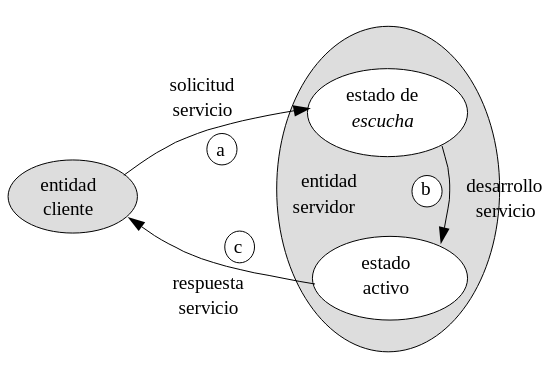
\includegraphics[width=0.5\textwidth]{images/cli-ser-1.png}
    \caption{Esquema de la arquitectura cliente-servidor.}
    \label{fig:cliente-servidor}
\end{figure}

\subsection{El software TCP/IP como parte del sistema operativo}

El software TCP/IP es una pieza fundamental integrada en el sistema operativo. Este software proporciona una interfaz para que las aplicaciones puedan comunicarse a través de redes utilizando los protocolos TCP/IP. Las características principales son:

\begin{itemize}
    \item \textbf{Interacción mediante la interfaz socket:} Las aplicaciones acceden al software TCP/IP a través de una API consistente basada en llamadas al sistema. Esta interfaz es conocida como \emph{la interfaz socket}.
    \item \textbf{Definición independiente de los protocolos:} Aunque está diseñada para operar con TCP/IP, la definición de la interfaz socket no forma parte de ningún protocolo en particular, lo que permite flexibilidad en su implementación.
    \item \textbf{Diversas implementaciones disponibles:} Existen varias implementaciones de la interfaz socket adaptadas a diferentes sistemas operativos y entornos, entre las que se encuentran:
    \begin{itemize}
        \item \textbf{Berkeley Socket Distribution:} Una implementación histórica y ampliamente utilizada en sistemas Unix.
        \item \textbf{Winsock:} La versión de la interfaz socket diseñada para sistemas Windows.
        \item \textbf{Transport Layer Interface (TLI):} Otra alternativa desarrollada para proporcionar servicios de transporte en redes.
    \end{itemize}
\end{itemize}

\subsection{La interfaz socket (BSD)}

La interfaz \emph{socket} es una extensión de la gestión de entrada/salida (I/O) tradicional del sistema operativo, diseñada para habilitar conexiones en red. Sus conceptos clave son:

\begin{itemize}
    \item \textbf{Gestión de I/O en el sistema operativo:} La entrada/salida en el sistema operativo sigue el modelo básico de:
    \begin{itemize}
        \item Abrir (\texttt{open}): Inicia el acceso a un recurso.
        \item Leer/escribir (\texttt{read}/\texttt{write}): Opera sobre el recurso.
        \item Cerrar (\texttt{close}): Finaliza el acceso al recurso.
    \end{itemize}
    Estos pasos se implementan mediante llamadas al sistema (\texttt{syscalls}).
    \item \textbf{El descriptor de fichero:} Es un concepto esencial que representa un identificador único para el recurso abierto, como un archivo o una conexión de red.
    \item \textbf{Extensión a conexiones en red:} La interfaz socket amplía el modelo de I/O para incluir la gestión de conexiones en red. Esto requiere identificar los puntos finales de la comunicación, definidos por:
    \begin{itemize}
        \item Dirección IP local.
        \item Dirección IP remota.
        \item Puerto local.
        \item Puerto remoto.
    \end{itemize}
    \item \textbf{Definición de un socket:} Un socket es un descriptor que representa una transmisión a través de la cual una aplicación puede enviar y/o recibir datos hacia y/o desde otro proceso de aplicación. Funciona como una “puerta” que conecta la aplicación con los servicios de transporte de red.
\end{itemize}

\subsubsection{Definición y estructura de un socket}

Un \emph{socket} es un concepto fundamental en la programación de redes y puede definirse como:

\begin{itemize}
    \item \textbf{Un descriptor de transmisión:} Representa una conexión a través de la cual una aplicación puede enviar y/o recibir información hacia y/o desde otro proceso de aplicación.
    \item \textbf{Puerta de acceso a los servicios de transporte:} Metafóricamente, un socket actúa como una “puerta” que conecta la aplicación con los servicios de transporte de red, facilitando la comunicación.
    \item \textbf{Implementación práctica:} En la práctica, un socket es una variable de tipo puntero a una estructura que contiene toda la información necesaria para gestionar la conexión, incluyendo los identificadores de los puntos finales (direcciones IP, puertos, etc.).
\end{itemize}

\subsection{Operaciones básicas con sockets}

En esta sección se describen las funciones y estructuras clave utilizadas para configurar y operar con sockets en la programación de redes.

\subsubsection{Especificar dirección IP y puerto local}

Para asociar un socket con una dirección IP y un puerto local, se utiliza la función \texttt{bind}:

\begin{verbatim}
int bind(int socket, struct sockaddr *myaddr, int addresslen);
\end{verbatim}

La dirección se pasa mediante la estructura \texttt{sockaddr\_in}:

\begin{verbatim}
struct sockaddr_in { /* Información de socket INET */
    short sin_family;       /* Familia: AF_INET */
    u_short sin_port;       /* Puerto: 16 bits, en orden de red */
    struct in_addr sin_addr; /* Dirección IP de 32 bits */
    char sin_zero[8];       /* No usada */
};
struct in_addr {
    u_long s_addr;          /* Dirección IP de 32 bits, en orden de red */
};
\end{verbatim}

Para usar esta estructura, es necesario realizar un \emph{casting}. Los campos incluyen:

\begin{itemize}
    \item \textbf{sin\_family:} Especifica la familia del protocolo, típicamente \texttt{AF\_INET}.
    \item \textbf{sin\_port:} Contiene el número de puerto.
    \item \textbf{sin\_addr:} Almacena la dirección IP.
\end{itemize}

\subsubsection{Especificar dirección IP y puerto remotos}

Para conectarse a un destino remoto, se utiliza la función \texttt{connect}:

\begin{verbatim}
int connect(int socket, struct sockaddr *toaddr, int addresslen);
\end{verbatim}

Dependiendo del tipo de socket:

\begin{itemize}
    \item \textbf{SOCK\_STREAM:} \texttt{connect} envía un SYN para iniciar el \emph{handshake} TCP, lo que requiere la simultaneidad de ambos procesos.
    \item \textbf{SOCK\_DGRAM:} No se envía nada a través de la red, pero se especifica la dirección IP y puerto remoto para facilitar el uso posterior.
\end{itemize}

\subsubsection{Poner un socket en modo pasivo}

Un servidor puede poner un socket en modo pasivo y definir el número de solicitudes pendientes en la cola con:

\begin{verbatim}
int listen(int sockfd, int maxwaiting);
\end{verbatim}

Esta llamada no es bloqueante. Para aceptar una conexión y detener el flujo del programa hasta que llegue una solicitud, se usa:

\begin{verbatim}
int accept(int sockfd, struct sockaddr *fromaddrptr, int *addresslen);
\end{verbatim}

\texttt{accept} devuelve un nuevo socket conectado para comunicarse con el cliente.

\subsubsection{Enviar y recibir datos}

\paragraph{Enviar datos:} Para enviar datos, se pueden utilizar:

\begin{verbatim}
int sendto(int sockfd, char *buff, int bufflen, int flags,
           struct sockaddr *toaddrptr, int addresslen);
int send(int sockfd, char *buff, int bufflen, int flags);
\end{verbatim}

\paragraph{Recibir datos:} Para recibir datos, se emplean las funciones:

\begin{verbatim}
int recvfrom(int sockfd, char *buff, int bufflen, int flags,
             struct sockaddr *fromaddrptr, int *addresslen);
int recv(int sockfd, char *buff, int bufflen, int flags);
\end{verbatim}

\subsubsection{Cerrar el socket}

Para cerrar un socket, se utilizan las funciones:

\begin{verbatim}
int close(int sockfd);
int shutdown(int sockfd, int how);
\end{verbatim}

\subsubsection{Otras funciones útiles}

Existen otras llamadas relacionadas con sockets y redes:

\begin{itemize}
    \item \texttt{read()}, \texttt{readv()}, \texttt{recvmsg()}
    \item \texttt{write()}, \texttt{writev()}, \texttt{sendmsg()}
    \item \texttt{gethostbyname()}, \texttt{getservbyname()}, \texttt{getprotobyname()}
    \item \texttt{htons()}, \texttt{htonl()}, \texttt{ntohs()}, \texttt{ntohl()}
\end{itemize}

\subsubsection{Ficheros cabecera típicos}

Las funciones anteriores requieren incluir los siguientes ficheros cabecera:

\begin{itemize}
    \item \texttt{netinet/in.h}
    \item \texttt{sys/types.h}
    \item \texttt{sys/socket.h}
\end{itemize}

\subsection{Tipos de servidores}

Los servidores pueden clasificarse en diferentes categorías según criterios específicos. A continuación, se presentan los tipos principales:

\subsubsection{Criterios de clasificación}

\begin{itemize}
    \item \textbf{Orientados a conexión vs. No orientados a conexión:}\footnote{Para imágenes detalladas, accede a las diapositivas 9-11 del tema 5.} 
    \begin{itemize}
        \item \emph{Orientados a conexión:} Establecen y mantienen una conexión antes de transmitir datos, típicamente usando TCP.
        \item \emph{No orientados a conexión:} No requieren una conexión persistente, trabajando con paquetes independientes, típicamente usando UDP.
    \end{itemize}
    \item \textbf{Iterativos vs. Concurrentes:}
    \begin{itemize}
        \item \emph{Iterativos:} Atienden una solicitud a la vez, procesando las solicitudes de manera secuencial.
        \item \emph{Concurrentes:} Atienden múltiples solicitudes simultáneamente, generalmente mediante el uso de hilos o procesos.
    \end{itemize}
\end{itemize}

\subsubsection{Tipos específicos de servidores}

\paragraph{Servidor iterativo no orientado a conexión:} 
Este tipo de servidor procesa las solicitudes una por una y no establece una conexión persistente con el cliente. Es eficiente para aplicaciones que usan UDP.

\paragraph{Servidor iterativo orientado a conexión:} 
Este servidor también atiende las solicitudes de manera secuencial, pero utiliza TCP para establecer una conexión con el cliente antes de procesar la solicitud.

\paragraph{Servidores concurrentes orientados a conexión:} 
Estos servidores gestionan múltiples conexiones simultáneamente, lo que los hace ideales para aplicaciones que requieren manejar múltiples clientes en paralelo.

\paragraph{Servidores multiprotocolo con I/O asíncrona (select):} 
Un único proceso iterativo ofrece soporte para múltiples protocolos. Utiliza I/O asíncrona y técnicas como \texttt{select()} para gestionar múltiples conexiones en una sola ejecución.

\paragraph{Servidores multiservicio:} 
Estos servidores ofrecen múltiples servicios con concurrencia, permitiendo manejar diferentes tipos de solicitudes simultáneamente, a menudo mediante el uso de hilos o procesos separados para cada servicio.


\footnotetext{Para profundizar en el tema de implementación de un socket puedes revisar la implementación del mismo en las diapositivas 23-29 del tema 5, pero no es objeto evaluable de examen.}

\subsection{Estimación de retardos en cola utilizando la teoría de colas}

La teoría de colas es una herramienta matemática utilizada para modelar y analizar los tiempos de espera en sistemas donde los recursos son compartidos. En el caso de redes, puede aplicarse para estimar los retardos en cola en servidores y routers.

\subsubsection{Modelo M/M/1}

Un servidor se modela como un sistema \textbf{M/M/1}, que se caracteriza por:

\begin{itemize}
    \item \textbf{Llegadas Poisson:} Las solicitudes llegan al sistema siguiendo una distribución de Poisson con una tasa promedio de llegadas \(\lambda\).
    \item \textbf{Tiempo de servicio exponencial:} El tiempo de servicio de las solicitudes sigue una distribución exponencial con tiempo promedio \(T_s\).
    \item \textbf{Un único servidor:} El sistema cuenta con un único recurso para procesar las solicitudes.
\end{itemize}

\subsubsection{Fórmula del retardo en cola}

El retardo promedio en cola (\(R\)) en un sistema M/M/1 puede calcularse con la siguiente fórmula:

\[
R = \frac{T_s \cdot \lambda}{1 - \lambda \cdot T_s}
\]

\begin{itemize}
    \item \(T_s\): Tiempo promedio de servicio.
    \item \(\lambda\): Tasa promedio de llegadas de solicitudes.
    \item El denominador \(1 - \lambda \cdot T_s\) refleja la relación entre la capacidad del servidor y la carga del sistema.
\end{itemize}

\subsubsection{Aplicación en routers}

Esta misma fórmula puede utilizarse para calcular el retardo en cola en un \textbf{router}, considerando las llegadas de paquetes y el tiempo necesario para procesarlos.

\begin{itemize}
    \item \textbf{Ejemplo:} Si un router procesa paquetes con un tiempo promedio de servicio \(T_s\) y recibe paquetes a una tasa de \(\lambda\), el retardo promedio en cola puede calcularse utilizando la expresión anterior.
\end{itemize}

\subsection{Definición y características de un protocolo de aplicación}

Un protocolo de aplicación define las reglas y mecanismos mediante los cuales dos procesos se comunican en una red. Los aspectos principales que caracterizan un protocolo de aplicación incluyen:

\subsubsection{Aspectos clave de un protocolo de aplicación}

\begin{itemize}
    \item \textbf{Tipo de servicio:} 
    \begin{itemize}
        \item \emph{Orientado o no orientado a conexión.}
        \item \emph{Realimentado o no realimentado.}
    \end{itemize}
    
    \item \textbf{Tipo de mensaje:}
    \begin{itemize}
        \item \emph{Request}, \emph{response}, entre otros.
    \end{itemize}
    
    \item \textbf{Sintaxis:} 
    Define y estructura los “campos” en el mensaje.
    \begin{itemize}
        \item En aplicaciones generalmente son orientados a texto (ej., HTTP).
        \item Excepciones: algunos protocolos como DNS.
        \item Tendencia: usar formato \emph{Type-Length-Value (TLV)}.
    \end{itemize}
    
    \item \textbf{Semántica:} 
    Define el significado de los campos.
    
    \item \textbf{Reglas:} 
    Especifican cuándo los procesos deben enviar mensajes o responder a mensajes.
\end{itemize}

\subsubsection{Tipos de protocolos}

\begin{itemize}
    \item \textbf{Según propiedad:} 
    \begin{itemize}
        \item \emph{Dominio público:} Definidos en RFCs (ej., HTTP, SMTP).
        \item \emph{Propietarios:} No estandarizados públicamente (ej., Skype, IGRP).
    \end{itemize}
    
    \item \textbf{Según la transmisión:}
    \begin{itemize}
        \item \emph{In-band:} Los datos y el control viajan juntos.
        \item \emph{Out-of-band:} Los datos y el control viajan por canales separados.
    \end{itemize}
    
    \item \textbf{Según estado:}
    \begin{itemize}
        \item \emph{Stateless:} No mantienen información de estado entre transacciones.
        \item \emph{Stateful:} Mantienen información de estado.
    \end{itemize}
    
    \item \textbf{Según persistencia:}
    \begin{itemize}
        \item \emph{Persistentes:} Mantienen la conexión abierta entre transacciones.
        \item \emph{No persistentes:} Cierran la conexión después de cada transacción.
    \end{itemize}
\end{itemize}

\subsubsection{Tendencias en los protocolos de aplicación}

Los protocolos modernos tienden a ser flexibles mediante:

\begin{itemize}
    \item Una \textbf{cabecera fija}.
    \item Una serie de \textbf{trozos} que pueden ser:
    \begin{itemize}
        \item Obligatorios u opcionales.
        \item Con cabeceras específicas más datos en forma de parámetros.
    \end{itemize}
\end{itemize}

\textbf{Formato TLV (Type-Length-Value):} 
\begin{itemize}
    \item Parámetros fijos (en orden).
    \item Parámetros de longitud variable u opcionales.
\end{itemize}

\begin{figure}[H]
    \centering
    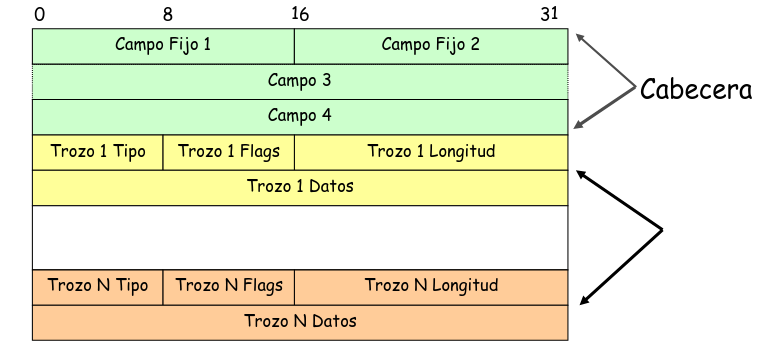
\includegraphics[width=0.8\textwidth]{images/aplicacion-img1.png}
    \caption{Estructura flexible en protocolos de aplicación.}
    \label{fig:protocolo-aplicacion}
\end{figure}

\subsection{Características y requisitos de las aplicaciones}

Las aplicaciones de red tienen diferentes características y requisitos según sus necesidades de funcionamiento. A continuación se describen algunos de los aspectos más importantes:

\begin{itemize}
    \item \textbf{Tolerancia a pérdidas de datos (errores):} 
    Algunas aplicaciones pueden tolerar la pérdida de datos sin afectar significativamente su rendimiento, como en el caso de aplicaciones de audio. En cambio, otras aplicaciones, como FTP, Telnet o HTTP, requieren una transferencia de datos completamente fiable.
    
    \item \textbf{Exigencia de requisitos temporales:}
    Las aplicaciones inelásticas, como la telefonía por Internet y los juegos interactivos, requieren un retardo (delay) acotado para ser efectivas. Otras aplicaciones, en cambio, no tienen estrictos requisitos de tiempo y pueden tolerar mayores retardos sin afectar la experiencia del usuario.
    
    \item \textbf{Demanda de ancho de banda (tasa de transmisión o throughput):}
    Algunas aplicaciones requieren un ancho de banda constante o una tasa de transmisión específica, como los códecs de vídeo. Otras aplicaciones, como la navegación web, pueden ser más flexibles en cuanto a la cantidad de datos transmitidos.
    
    \item \textbf{Nivel de seguridad:}
    Los requisitos de seguridad varían entre aplicaciones. Algunas pueden necesitar características avanzadas como encriptación, autenticación, no repudio e integridad de los datos, mientras que otras tienen requisitos de seguridad más bajos.
\end{itemize}

\subsubsection{Conclusión}

En resumen, las distintas aplicaciones tienen requisitos heterogéneos, lo que significa que no existe un único estándar que se adapte a todas las aplicaciones. Estos requisitos deben ser gestionados adecuadamente para garantizar un funcionamiento eficiente y seguro de las aplicaciones de red.


\subsection{Requerimientos de algunas aplicaciones}

\begin{figure}[H]
    \centering
    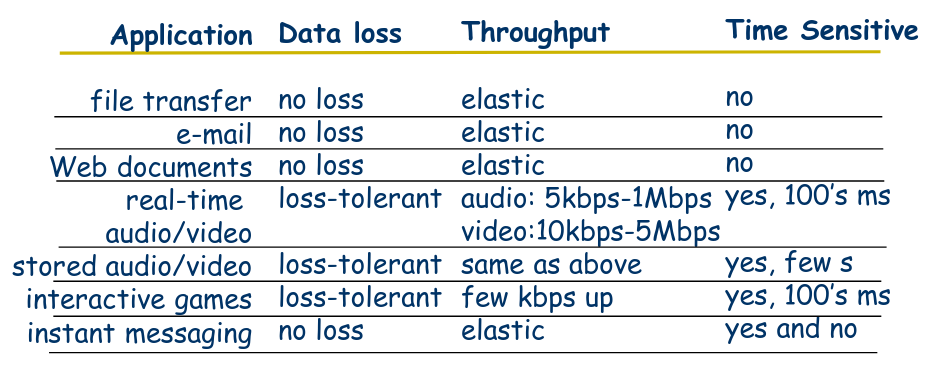
\includegraphics[width=0.8\textwidth]{images/requerimientos.png}
    \caption{Requerimientos de algunas aplicaciones.}
    \label{fig:requerimientos-aplicaciones}
\end{figure}

\subsection{Protocolos de Transporte}

Los protocolos de transporte son fundamentales para la comunicación en redes, ya que gestionan la transferencia de datos entre aplicaciones en diferentes dispositivos. Dos de los protocolos más utilizados en esta capa son \textbf{TCP} y \textbf{UDP}.

\subsubsection{Introducción a las aplicaciones de red}

TCP y UDP, como protocolos de la capa de transporte, se apoyan en el protocolo IP de la capa de red. Sin embargo, es importante destacar que no garantizan \emph{Calidad de Servicio} (QoS), lo que significa que:

\begin{itemize}
    \item El \textbf{retardo no está acotado}.
    \item Las \textbf{fluctuaciones en el retardo no están acotadas}.
    \item No hay una \textbf{velocidad de transmisión mínima garantizada}.
    \item No existe una \textbf{probabilidad de pérdidas acotada}.
    \item Tampoco hay garantías de \textbf{seguridad}.
\end{itemize}

\subsubsection{Servicio TCP}

El protocolo TCP (Transmission Control Protocol) ofrece un servicio \textbf{orientado a conexión} que garantiza un transporte fiable, es decir, asegura que los datos lleguen sin errores y en el orden correcto. Sus características incluyen:

\begin{itemize}
    \item \textbf{Transporte fiable con control de errores.}
    \item \textbf{Control de flujo.} Asegura que el receptor no sea sobrecargado con datos.
    \item \textbf{Control de congestión.} Ajusta la cantidad de datos enviados para evitar la congestión en la red.
\end{itemize}

\subsubsection{Servicio UDP}

El protocolo UDP (User Datagram Protocol), en contraste con TCP, es \textbf{no orientado a conexión} y no garantiza la fiabilidad en la transmisión de datos. Sus características incluyen:

\begin{itemize}
    \item \textbf{Transporte no fiable.} Los datos pueden perderse sin ser retransmitidos.
    \item \textbf{Sin control de flujo.} No hay mecanismos para regular la cantidad de datos que se envían.
    \item \textbf{Sin control de congestión.} No hay medidas para prevenir la sobrecarga en la red.
\end{itemize}

\subsubsection{¿Para qué existe UDP?}

UDP es útil en situaciones donde la rapidez es más importante que la fiabilidad, como en aplicaciones de streaming de video, voz sobre IP (VoIP) y juegos en línea, donde la transmisión rápida de datos es crucial y se puede tolerar alguna pérdida de información.

\begin{figure}[H]
    \centering
    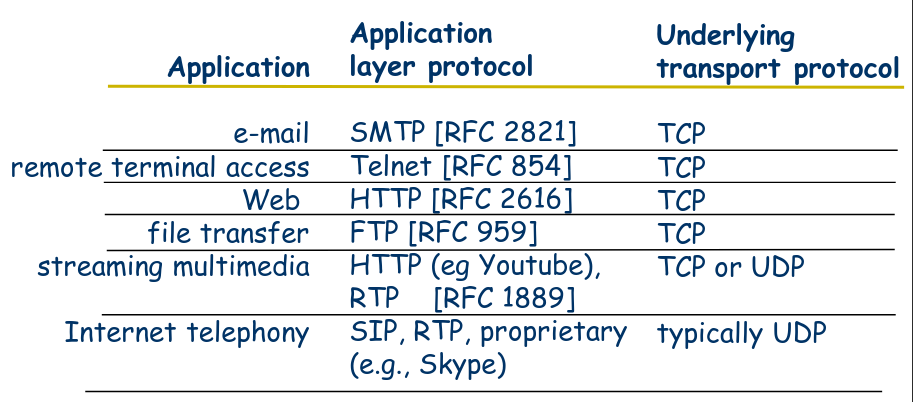
\includegraphics[width=0.8\textwidth]{images/protocolos-transporte.png}
    \caption{Comparación de los servicios TCP y UDP.}
    \label{fig:protocolos-transporte}
\end{figure}

\section{Servicio de Nombres de Dominio (DNS)}

\subsection{La comunicación en Internet y las direcciones IP}

La comunicación en Internet depende de las direcciones IP para identificar a los dispositivos y permitir la transmisión de datos. Sin embargo, los usuarios prefieren utilizar \textbf{nombres de dominio}, ya que son mucho más fáciles de recordar que una dirección IP numérica. Actualmente, existen más de 300 millones de nombres de dominio registrados.

\subsubsection{Sistema de nombres de dominio (DNS)}

El \textbf{DNS} (Domain Name System) es el sistema que permite traducir los nombres de dominio a direcciones IP, un proceso conocido como \emph{resolución de nombres}. Por ejemplo, el nombre de dominio \texttt{dns.ugr.es} se traduce a la dirección IP \texttt{150.214.204.10}.

\subsubsection{Estructura jerárquica de los dominios}

El sistema de nombres de dominio tiene una estructura jerárquica, donde los dominios se organizan de la siguiente manera:

\[
\text{Parte\_local.dominio\_nivel1.}\dots.\text{dominio\_nivel2.dominio\_nivel1.}
\]

El \textbf{dominio de nivel 1} es el más cercano al final y generalmente es un dominio genérico, como \texttt{.com}, \texttt{.es}, \texttt{.edu}, etc.

El \textbf{dominio raíz} o \texttt{.} es el nivel más alto de la jerarquía y es gestionado por \textbf{ICANN} (Internet Corporation for Assigned Names and Numbers). ICANN delega la gestión de algunos dominios genéricos a centros regionales de autoridad.

\subsubsection{Dominios genéricos}

Inicialmente, se definieron los siguientes nueve dominios genéricos en el RFC 1591:

\begin{itemize}
    \item \texttt{.com} -> Organizaciones comerciales.
    \item \texttt{.edu} -> Instituciones educativas, como universidades, en los Estados Unidos.
    \item \texttt{.gov} -> Instituciones gubernamentales de los Estados Unidos.
    \item \texttt{.mil} -> Organizaciones militares de los Estados Unidos.
    \item \texttt{.net} -> Proveedores de Internet.
    \item \texttt{.org} -> Organizaciones diversas que no encajan en las categorías anteriores.
    \item \texttt{.arpa} -> Usado para propósitos exclusivos de infraestructura de Internet.
    \item \texttt{.int} -> Organizaciones establecidas por tratados internacionales entre gobiernos.
    \item \texttt{.xy} -> Indicativos de zona geográfica, como \texttt{.es} para España, \texttt{.pt} para Portugal, \texttt{.jp} para Japón, etc.
\end{itemize}

\subsubsection{Lecturas recomendadas}

Para profundizar más sobre el tema de los nombres de dominio y el sistema DNS, se recomienda la siguiente documentación:

\begin{itemize}
    \item \textbf{Tutorial sobre "Los nombres de dominios":} \url{https://www.icann.org/en/system/files/files/domain-names-beginners-guide-06dec10-es.pdf}
    \item \textbf{Instrucciones para registrar un nombre de dominio en .es:} \url{https://www.dominios.es/es/registra-un-dominio/como-registrar-dominio}
    \item \textbf{Instalación y ejemplos de ficheros de configuración de \texttt{named}:} \url{https://www.tldp.org/HOWTO/DNS-HOWTO.html}
\end{itemize}


\subsection{DNS: Protocolo de aplicación para la resolución de nombres}

DNS (Domain Name System) es un protocolo de aplicación utilizado para acceder a una base de datos distribuida que gestiona la resolución de nombres en Internet. Este protocolo permite traducir los nombres de dominio a direcciones IP, facilitando la comunicación entre los dispositivos de la red.

\subsubsection{Niveles de servidores DNS}

El sistema DNS se organiza en tres niveles de servidores, que gestionan la resolución de nombres de dominio:

\begin{itemize}
    \item \textbf{Servidores raíz (\texttt{.})}: Son los servidores más altos en la jerarquía de DNS y gestionan la información sobre los servidores de dominio de nivel superior (TLD).
    \item \textbf{Servidores de dominio (\texttt{TLD})}: Estos servidores gestionan los dominios de nivel superior como \texttt{.com}, \texttt{.org}, \texttt{.edu}, etc.
    \item \textbf{Servidores locales}: Son servidores DNS específicos para una red local o proveedor de servicios de Internet, encargados de resolver las consultas locales de los usuarios.
\end{itemize}

\subsubsection{Proceso de resolución de nombres}

Cuando un usuario quiere acceder a un sitio web como \texttt{jcp.ugr.es} o \texttt{www.google.com}, el proceso de resolución de nombres sigue estos pasos:

\begin{enumerate}
    \item El \textbf{resolver local} realiza una consulta para resolver el nombre de dominio.
    \item Se establece una conexión con el servidor DNS local, cuyo IP es conocida previamente.
    \item El servidor DNS local lleva a cabo la resolución del nombre de dominio.
\end{enumerate}

\subsubsection{Tipos de resolución}

Existen dos tipos de resolución que se utilizan en el proceso de obtención de la dirección IP asociada a un nombre de dominio:

\begin{itemize}
    \item \textbf{Resolución iterativa}: El servidor DNS responde con la mejor información disponible, indicando a la aplicación que consulte otros servidores si es necesario.
    \item \textbf{Resolución recursiva}: El servidor DNS se encarga de realizar todas las consultas necesarias hasta encontrar la respuesta completa y devolverla al cliente.
\end{itemize}

\subsubsection{Mejoras en el rendimiento: Uso de caches}

Para mejorar el rendimiento y reducir el tiempo de respuesta, los servidores DNS utilizan \textbf{caches} para almacenar las respuestas a las consultas más frecuentes. De esta manera, si un nombre de dominio ha sido resuelto recientemente, el servidor puede devolver la dirección IP almacenada en lugar de realizar una consulta a los servidores superiores\footnote{Para más imágenes consulte la diapositiva 43 del tema 5.}.

\begin{figure}[H]
    \centering
    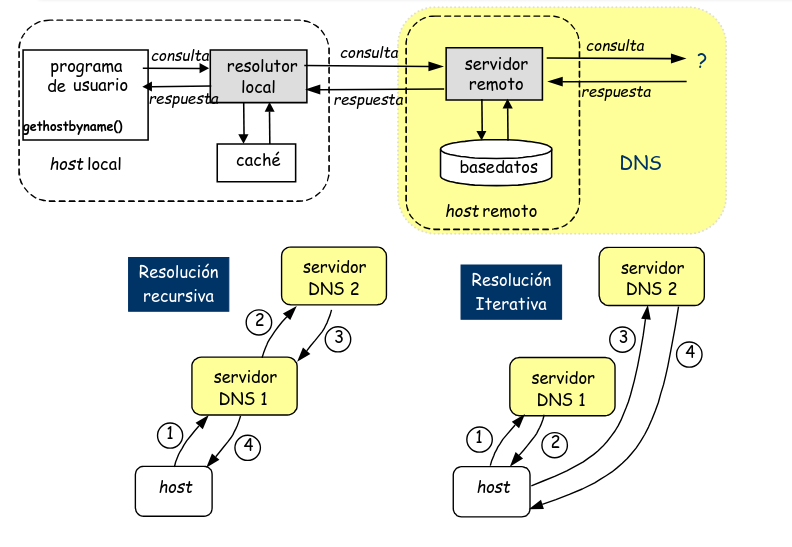
\includegraphics[width=0.8\textwidth]{images/dns.png}
    \caption{Esquema del funcionamiento del sistema DNS.}
    \label{fig:dns}
\end{figure}

\subsection{Gestión de la base de datos distribuida y jerárquica en DNS}

El sistema DNS está formado por una base de datos distribuida y jerárquica, gestionada por un conjunto de servidores cooperativos que almacenan parcialmente la información. Esta base de datos se denomina \textbf{BIND} (Berkeley Internet Name Domain). 

\subsubsection{Zonas en DNS}

Cada servidor DNS es responsable de una \textbf{zona}. Una zona es un conjunto de nombres de dominio contiguos dentro de un nodo del árbol DNS. El servidor tiene toda la información sobre esa zona y es considerado su autoridad.

\begin{itemize}
    \item \textbf{Servidor de autoridad (SOA, Start of Authority)}: Los servidores de autoridad deben contener toda la información de su zona, no solo la cacheada.
    \item \textbf{Delegación jerárquica}: La autoridad puede delegarse a otros servidores en niveles más bajos de la jerarquía del DNS.
\end{itemize}

\subsubsection{Gestión de la base de datos DNS}

La gestión de la base de datos DNS se organiza de la siguiente manera:

\begin{itemize}
    \item Cada zona debe tener al menos un \textbf{servidor de autoridad}.
    \item En cada zona existen servidores \textbf{primarios}, que almacenan una copia maestra de la base de datos en discos locales, y servidores \textbf{secundarios}, que obtienen la base de datos por transferencia.
    \item Además, existe un servicio de \textbf{cache} para mejorar el rendimiento de las consultas.
\end{itemize}

\subsubsection{Topología de servidores DNS}

La topología real de los servidores DNS es compleja. Existen 13 servidores raíz, identificados por las letras A a M, que forman el núcleo de la infraestructura DNS global. Los servidores raíz tienen copias distribuidas de los datos, y algunos de ellos están ubicados en diferentes puntos del mundo, como en Madrid, en el punto neutro \texttt{Espanix}.

\subsubsection{Resolución de nombres por el resolver local}

Cuando un cliente realiza una consulta DNS a través de un \textbf{resolver local}, pueden ocurrir varios escenarios:

\begin{itemize}
    \item \textbf{Respuesta con autoridad}: El servidor tiene autoridad sobre la zona que contiene el nombre solicitado y devuelve la dirección IP correspondiente.
    \item \textbf{Respuesta sin autoridad}: El servidor no tiene autoridad sobre la zona solicitada, pero tiene la respuesta almacenada en su cache.
    \item \textbf{No conoce la respuesta}: El servidor consulta otros servidores de forma recursiva o iterativa. Normalmente, la petición se eleva a uno de los servidores raíz.
\end{itemize}

\subsubsection{Servidores raíz DNS}

Los servidores raíz DNS son gestionados por diferentes organizaciones alrededor del mundo. A continuación, se enumeran algunos de los servidores raíz:

\begin{itemize}
    \item \textbf{Servidor A}: Network Solutions, Herndon, Virginia, USA.
    \item \textbf{Servidor B}: Instituto de Ciencias de la Información de la Universidad del Sur de California, USA.
    \item \textbf{Servidor C}: PSINet, Virginia, USA.
    \item \textbf{Servidor D}: Universidad de Maryland, USA.
    \item \textbf{Servidor E}: NASA, Mountain View, California, USA.
    \item \textbf{Servidor F}: Internet Software Consortium, Palo Alto, California, USA.
    \item \textbf{Servidor G}: Agencia de Sistemas de Información de Defensa, California, USA.
    \item \textbf{Servidor H}: Laboratorio de Investigación del Ejército, Maryland, USA.
    \item \textbf{Servidor I}: NORDUnet, Estocolmo, Suecia.
    \item \textbf{Servidor J}: (TBD), Virginia, USA.
    \item \textbf{Servidor K}: RIPE-NCC, Londres, Inglaterra.
    \item \textbf{Servidor L}: (TBD), California, USA.
    \item \textbf{Servidor M}: Wide Project, Universidad de Tokyo, Japón.
\end{itemize}

\subsection{Base de datos DNS}

En el sistema DNS, todo dominio está asociado al menos a un \textbf{registro de recurso} (Resource Record, RR). Cada RR es una tupla con cinco campos:

\begin{itemize}
    \item \textbf{Nombre del dominio}: El nombre del dominio al que se refiere el registro.
    \item \textbf{Tiempo de vida}: Tiempo de validez del registro, utilizado para la cache de las consultas.
    \item \textbf{Clase}: En Internet, siempre es \texttt{IN} (Internet).
    \item \textbf{Tipo}: El tipo de registro, que define el propósito del RR.
    \item \textbf{Valor}: El contenido que depende del tipo de registro.
\end{itemize}

Los tipos de registros más comunes son:

\begin{itemize}
    \item \textbf{SOA (Start Of Authority)}: Indica la autoridad de la zona.
    \item \textbf{NS (Name Server)}: Contiene información sobre los servidores de nombres de la zona.
    \item \textbf{A (Address)}: Define una dirección IPv4 asociada a un nombre de dominio.
    \item \textbf{MX (Mail Exchange)}: Define un servidor de correo electrónico para el dominio.
    \item \textbf{CNAME (Canonical Name)}: Define el nombre canónico de un nombre de dominio.
    \item \textbf{HINFO (Host Information)}: Contiene información sobre el tipo de máquina y el sistema operativo.
    \item \textbf{TXT (Text)}: Contiene información textual sobre el dominio.
\end{itemize}

Además, existe una base de datos asociada de \textbf{resolución inversa} para traducir direcciones IP en nombres de dominio. Esta base de datos se encuentra bajo el dominio \texttt{in-addr.arpa}\footnote{Ejemplos de estos registros se encuentran en la diapositiva 49 del Tema 5.}.

\subsection{Formato de mensajes DNS}

DNS generalmente utiliza el puerto 53 y se comunica a través de \textbf{UDP}, aunque utiliza \textbf{TCP} para respuestas grandes (cuando el tamaño de la respuesta es mayor a 512 bytes). 

Para más información, se pueden consultar los siguientes documentos:

\begin{itemize}
    \item RFC 1034 y RFC 1035 (actualizados por los RFC 3597 y 3658)
    \item \texttt{/usr/doc/HOWTO/trans/es/DNS-COMO}
    \item Comandos como \texttt{man named}, \texttt{nslookup}, \texttt{resolver}, \texttt{host.conf}, \texttt{dig}
    \item DNSSEC: \url{http://www.dominios.es/dominios/sites/dominios/files/1318333648229_0.pdf}
\end{itemize}

\begin{figure}[H]
    \centering
    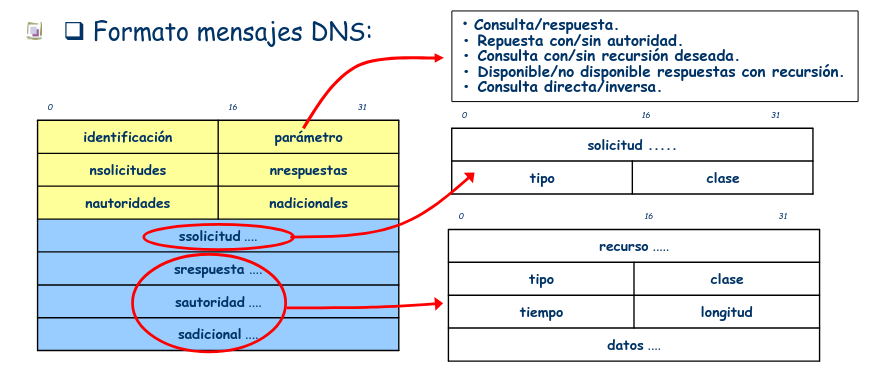
\includegraphics[width=\textwidth]{images/msg-dns.png}
    \caption{Formato de mensajes DNS}
\end{figure}

\subsubsection{Ejemplo de solicitud DNS}

En la siguiente figura, se ilustra un ejemplo de acceso DNS por parte de una máquina (\texttt{jcp.ugr.es}) que desea acceder a los servicios de \texttt{www.google.com}. Para obtener la dirección IP del servidor, la consulta debe pasar por varios servidores, como se muestra en el gráfico.

\begin{figure}[H]
    \centering
    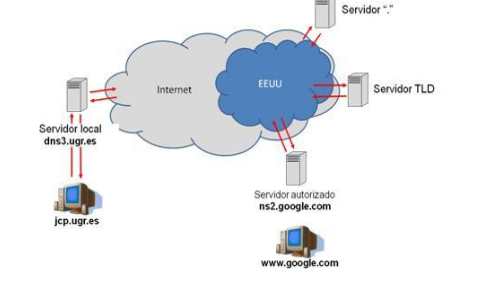
\includegraphics[width=\textwidth]{images/dns-ej.png}
    \caption{Ejemplo de acceso DNS de jcp.ugr.es a www.google.com}
\end{figure}

Supongamos que se consideran los siguientes retardos promedio:
\begin{itemize}
    \item 8 $\mu$s dentro de una red LAN.
    \item 12 ms por cada acceso a través de Internet.
    \item 1 ms de procesamiento en cada servidor.
    \item 4 ms si la conexión se restringe a EE. UU.
\end{itemize}

Para calcular el tiempo que se tarda en procesar la solicitud bajo dos políticas diferentes de consulta, realizamos los siguientes cálculos:

\paragraph{1. Solicitud recursiva al servidor local, pero el servidor realiza solicitudes iterativas:}
En este caso, la solicitud recursiva al servidor local implica que el servidor local debe realizar consultas a otros servidores de forma iterativa. Considerando los servidores involucrados en la jerarquía de DNS (servidores raíz, servidores TLD, y servidores autoritativos), se suman los retardos asociados con cada acceso.

\begin{itemize}
    \item Retardo en la LAN (8 $\mu$s).
    \item 1 ms de procesamiento en el servidor local.
    \item 12 ms por cada acceso a través de Internet para llegar a un servidor de nivel superior.
    \item 1 ms de procesamiento adicional en cada servidor intermedio.
\end{itemize}

La suma total para cada nivel de servidor debe repetirse dependiendo de cuántos servidores estén involucrados en la consulta (de acuerdo con el gráfico). Los tiempos de acceso se acumulan a medida que el servidor local hace las consultas iterativas.

\paragraph{2. Solicitud iterativa directamente a los servidores raíz:}
En este caso, el servidor local no realiza consultas recursivas. El cliente consulta directamente a los servidores raíz, lo que reduce el número de pasos involucrados en la resolución.

En este caso, se puede deducir que el tiempo total se reduce debido a que el servidor local no realiza múltiples consultas.

\subsubsection{Comparación y desventajas}
La política \textbf{recursiva} es más lenta debido a que cada servidor debe realizar consultas adicionales para resolver el nombre. En cambio, la política \textbf{iterativa} es más rápida porque el cliente directamente consulta a los servidores raíz y TLD.

Sin embargo, la desventaja de la política iterativa es que depende de la capacidad del cliente para manejar las consultas directamente a los servidores autoritativos. Además, la política iterativa puede resultar menos eficiente si el cliente no tiene configuraciones adecuadas para realizar consultas directas a varios servidores.

\section{Navegación Web}

\subsection{Páginas Web y HTTP}

Una página web es un archivo (generalmente en formato \texttt{HTML}) que está formado por diversos objetos, tales como:

\begin{itemize}
    \item \textbf{Archivos HTML}
    \item \textbf{Imágenes} (por ejemplo, en formato JPEG)
    \item \textbf{Applets de Java}
    \item \textbf{Archivos de audio}
    \item \textbf{Archivos de vídeo}
\end{itemize}

Cada objeto dentro de la página web es direccionado a través de una \textbf{URL (Uniform Resource Locator)} o \textbf{URI (Uniform Resource Identifier)}. El formato de la URL sigue una estructura estándar, que puede desglosarse de la siguiente manera:

\begin{itemize}
    \item \texttt{[usuario[:contrase\~na]@]dominio[:puerto][/ruta][/recurso][?solicitud][\#fragmento]}
\end{itemize}

\subsection{Protocolo HTTP}
Las páginas web se sirven a través del protocolo \textbf{HTTP (Hypertext Transfer Protocol)}, que es un protocolo \textbf{cliente-servidor}. En este modelo:

\begin{itemize}
    \item \textbf{Cliente}: Generalmente un navegador web (como Google Chrome, Firefox, etc.), que realiza una solicitud, recibe y muestra los objetos web.
    \item \textbf{Servidor}: Un servidor web, que recibe las solicitudes del cliente y responde enviando los objetos web correspondientes.
\end{itemize}

Las páginas web pueden clasificarse en dos tipos:

\begin{enumerate}
    \item \textbf{Estáticas}: El contenido de estas páginas no cambia. Son simples y contienen los mismos datos para cada usuario.
    \item \textbf{Dinámicas}: Estas páginas pueden cambiar su contenido en función de factores como la interacción del usuario, la hora, los datos extraídos de bases de datos, entre otros.
\end{enumerate}

\subsection{Páginas Dinámicas}
Las páginas dinámicas generan contenido variable utilizando:

\begin{itemize}
    \item \textbf{Lenguajes de scripting en el cliente}: Como \texttt{JavaScript} o \texttt{Flash}, que son ejecutados en el navegador del cliente.
    \item \textbf{Lenguajes de scripting en el servidor}: Como \texttt{Perl}, \texttt{PHP}, \texttt{Ruby}, \texttt{Python}, que se utilizan para procesar las solicitudes del cliente en el servidor, insertando contenido dinámico, como resultados de consultas a bases de datos. Estos lenguajes permiten incrustar etiquetas dentro del código HTML, y cuando el servidor recibe la solicitud, interpreta estas etiquetas para generar contenido dinámico.
\end{itemize}

\subsection{Características de HTTP}

\begin{itemize}
    \item \textbf{Puerto de conexión}: HTTP utiliza el servicio de \textbf{TCP (Transmission Control Protocol)} en el puerto \texttt{80}. Esto significa que la comunicación entre el cliente y el servidor se realiza a través de conexiones TCP.
    \item \textbf{Modelo de Conexión}:
    \begin{enumerate}
        \item \textbf{Inicio de Conexión TCP}: El cliente establece la conexión con el servidor.
        \item \textbf{Envío de solicitud HTTP}: El cliente realiza una solicitud HTTP al servidor.
        \item \textbf{Cierre de Conexión TCP}: Después de que el servidor envía la respuesta al cliente, la conexión TCP se cierra.
    \end{enumerate}
    \item \textbf{HTTP es "stateless"}: Esto significa que \textbf{HTTP no guarda el estado} de la sesión del cliente. Cada solicitud es independiente de las anteriores, lo que ahorra recursos en el servidor. Sin embargo, esto hace que la interacción entre el cliente y el servidor sea más compleja, ya que el servidor no mantiene ninguna información sobre las solicitudes previas. Para manejar el estado, se utilizan tecnologías como las \textbf{cookies}, que permiten a los servidores almacenar pequeños fragmentos de información en el navegador del cliente.
\end{itemize}

\subsection{Tipos de Servidores HTTP}
Existen dos tipos principales de servidores HTTP:

\begin{enumerate}
    \item \textbf{Servidores No Persistentes}: En este tipo de servidores, solo se envía un objeto por cada conexión TCP. Esto significa que cada vez que el cliente solicita un nuevo objeto (por ejemplo, una imagen o un archivo HTML), se establece una nueva conexión TCP entre el cliente y el servidor.
    \item \textbf{Servidores Persistentes}: En estos servidores, se pueden enviar múltiples objetos a través de una sola conexión TCP entre el cliente y el servidor. Esto mejora la eficiencia y reduce el tiempo necesario para cargar una página web, ya que no es necesario establecer una nueva conexión TCP para cada objeto solicitado.
\end{enumerate}

\subsection{Mensajes HTTP}
\begin{enumerate}
    \item El cliente HTTP (navegador) solicita un objeto identificado por su URL, en el ejemplo \texttt{www.ugr.es/pages/Universidad}. Según la configuración del servidor, si no se especifica nada, por defecto se sirve el fichero \texttt{index.html}.
    \item El cliente consulta al resolver de DNS por la dirección IP de \texttt{www.ugr.es}.
    \item DNS contesta \texttt{150.214.27.71} (IP virtual de un servicio balanceado).
    \item El cliente abre una conexión TCP al puerto 80 de \texttt{150.214.27.71} (3 bandas).
    \item El cliente envía una petición \texttt{GET /pages/universidad/ ...} (más otra información adicional: cabeceras, cookies, variables, etc).
    \item El servidor responde enviando el fichero \texttt{index.html} por la misma conexión TCP.
    \item Al usar TCP, el cliente y servidor de HTTP reciben un servicio orientado a conexión, fiable, sin errores, con control de flujo, con control de congestión, etc. Es decir, una comunicación TRANSPARENTE y FIABLE.
    \item Si es persistente, se siguen solicitando objetos de la página (\texttt{GET ...}) por la conexión.
    \item Se cierra la conexión TCP y se liberan recursos en el servidor y cliente.
    \item El cliente visualiza el contenido.
\end{enumerate}

\begin{figure}[H]
    \centering
    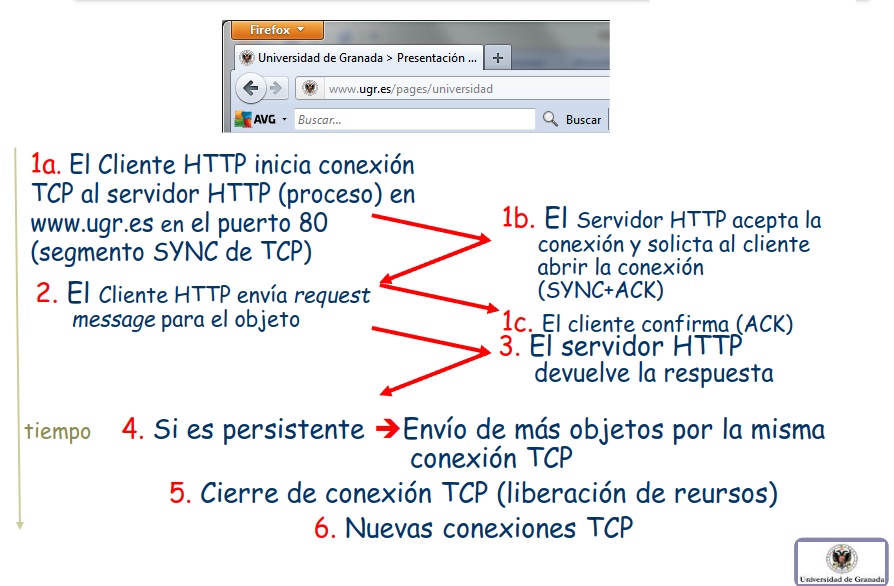
\includegraphics[width=0.8\textwidth]{images/nav_web.png}
    \caption{Ejemplo de comunicación HTTP.}
\end{figure}

HTTP define dos tipos de mensajes principales: las solicitudes del cliente al servidor (request) y las respuestas del servidor al cliente (response).

\subsubsection{HTTP Request Message (Solicitud del Cliente al Servidor)}

Un mensaje de solicitud HTTP enviado por el cliente al servidor tiene la siguiente estructura:

\begin{verbatim}
GET /somedir/page.html HTTP/1.1
Host: www.someschool.edu
User-agent: Mozilla/4.0
Connection: close
Accept-language: fr
\end{verbatim}

\begin{itemize}
    \item \textbf{Línea de petición:} Esta línea contiene el método HTTP (en este caso, \texttt{GET}), el recurso solicitado (\texttt{/somedir/page.html}) y la versión del protocolo HTTP (\texttt{HTTP/1.1}).
    \item \textbf{Líneas de cabecera:} Estas líneas contienen información adicional sobre la solicitud, como el host (\texttt{Host: www.someschool.edu}), el agente de usuario (\texttt{User-agent: Mozilla/4.0}), el tipo de conexión (\texttt{Connection: close}) y el idioma aceptado (\texttt{Accept-language: fr}).
    \item \textbf{Carriage Return + Line Feed (CRLF):} Indican el fin del mensaje.
\end{itemize}

\subsubsection{HTTP Response Message (Respuesta del Servidor al Cliente)}

Un mensaje de respuesta HTTP enviado por el servidor al cliente tiene la siguiente estructura:

\begin{verbatim}
HTTP/1.1 200 OK
Connection: close
Date: Thu, 06 Aug 1998 12:00:15 GMT
Server: Apache/1.3.0 (Unix)
Last-Modified: Mon, 22 Jun 1998
Content-Length: 6821
Content-Type: text/html
data data data data data ...
\end{verbatim}

\begin{itemize}
    \item \textbf{Línea de estado:} Esta línea contiene la versión del protocolo HTTP (\texttt{HTTP/1.1}), el código de estado de la respuesta (\texttt{200 OK}) que indica que la solicitud fue exitosa, y una breve descripción del estado.
    \item \textbf{Líneas de cabecera:} Estas líneas contienen información adicional sobre la respuesta, como el tipo de conexión (\texttt{Connection: close}), la fecha en la que se generó la respuesta (\texttt{Date: Thu, 06 Aug 1998 12:00:15 GMT}), el servidor que está procesando la solicitud (\texttt{Server: Apache/1.3.0 (Unix)}), la última vez que el recurso fue modificado (\texttt{Last-Modified: Mon, 22 Jun 1998}) y el tipo de contenido (\texttt{Content-Type: text/html}).
    \item \textbf{Datos:} Finalmente, los datos del mensaje pueden ser el contenido solicitado, como el fichero HTML o cualquier otro recurso.
\end{itemize}

\subsection{Ejercicio: Comparación de rendimiento entre HTTP Persistente y No Persistente}

Considerando los siguientes parámetros:

\begin{itemize}
    \item \textbf{Descarga de una página web con 10 objetos incrustados}
    \item \textbf{Tiempo de Establecimiento de conexión TCP}: 5 ms
    \item \textbf{Tiempo de Cierre de conexión TCP}: 5 ms
    \item \textbf{Tiempo de Solicitud HTTP}: 2 ms
    \item \textbf{Tiempo de Respuesta HTTP}: 10 ms
\end{itemize}
\newpage
\subsubsection{HTTP No Persistente}
En HTTP no persistente, cada objeto se solicita en una conexión TCP separada. El tiempo por objeto es el siguiente:

\[
\text{Tiempo por objeto} = \text{Establecimiento de conexión} + \text{Solicitud HTTP} +
\]
\[
\text{Respuesta HTTP} + \text{Cierre de conexión}
\]
\[
\text{Tiempo por objeto} = 5 \, \text{ms} + 2 \, \text{ms} + 10 \, \text{ms} + 5 \, \text{ms} = 22 \, \text{ms}
\]

Dado que hay 10 objetos incrustados, el tiempo total de descarga será:

\[
\text{Tiempo total} = 10 \, \text{objetos} \times 22 \, \text{ms} = 220 \, \text{ms}
\]

\subsubsection{HTTP Persistente}
En HTTP persistente, todos los objetos se solicitan a través de una única conexión TCP. El tiempo por objeto es:

\[
\text{Tiempo por objeto} = 2 \, \text{ms} + 10 \, \text{ms} = 12 \, \text{ms}
\]

El tiempo total de descarga será:

\[
\text{Tiempo total} = \text{Establecimiento de conexión} + 10 \times \text{Tiempo por objeto} + \text{Cierre de conexión}
\]
\[
\text{Tiempo total} = 5 \, \text{ms} + 10 \times 12 \, \text{ms} + 5 \, \text{ms} = 5 \, \text{ms} + 120 \, \text{ms} + 5 \, \text{ms} = 130 \, \text{ms}
\]

\subsubsection{Solución}
\begin{itemize}
    \item \textbf{HTTP No Persistente}: Tiempo total = 220 ms
    \item \textbf{HTTP Persistente}: Tiempo total = 130 ms
\end{itemize}

\subsection{Métodos HTTP y Códigos de Respuesta}

\textbf{Métodos HTTP (acciones solicitadas por los clientes en los request messages):}
\begin{itemize}
    \item \textbf{OPTIONS:} Solicitud de información sobre las opciones disponibles en el servidor.
    \item \textbf{GET:} Solicitud de un recurso. Puede ser condicional.
    \item \textbf{HEAD:} Igual que GET pero el servidor no devuelve el cuerpo, solo las cabeceras.
    \item \textbf{POST:} Solicitud para que el servidor acepte y subordine los datos de la solicitud a la URI especificada.
    \item \textbf{PUT:} Solicitud para reemplazar la URI especificada con los datos incluidos en la solicitud.
    \item \textbf{DELETE:} Solicitud para borrar el recurso identificado por la URI.
\end{itemize}

\textbf{Códigos de Respuesta (para los response messages del servidor):}
\begin{itemize}
    \item \textbf{1xx:} Mensajes informativos.
    \item \textbf{2xx:} Indican éxito en la operación.
    \item \textbf{3xx:} Redirección, el cliente debe hacer algo más para completar la solicitud.
    \item \textbf{4xx:} Errores del cliente, como una solicitud mal formulada.
    \item \textbf{5xx:} Errores del servidor, el servidor no pudo completar la solicitud.
\end{itemize}

\textbf{Cabeceras comunes en HTTP:}
\begin{itemize}
    \item \textbf{Content-Type:} Describe el tipo MIME de la información contenida en el mensaje.
    \item \textbf{Content-Length:} Longitud en bytes de los datos enviados.
    \item \textbf{Content-Encoding:} Formato de codificación de los datos enviados (por ejemplo, compresión).
    \item \textbf{Date:} Fecha y hora de la operación.
\end{itemize}

\textbf{Cabeceras solo para peticiones del cliente:}
\begin{itemize}
    \item \textbf{Accept:} Tipos MIME aceptados por el cliente.
    \item \textbf{Authorization:} Clave de acceso para acceder a recursos protegidos.
    \item \textbf{From:} Dirección de correo electrónico del usuario que realiza la petición.
    \item \textbf{If-Modified-Since:} Permite operaciones GET condicionales según la fecha de modificación del objeto.
    \item \textbf{Referer:} URL del documento que activó el enlace.
    \item \textbf{User-Agent:} Identifica el tipo y versión del cliente que realiza la petición.
\end{itemize}

\textbf{Cabeceras solo para respuestas del servidor HTTP:}
\begin{itemize}
    \item \textbf{Allow:} Métodos HTTP opcionales que se pueden aplicar sobre el objeto.
    \item \textbf{Expires:} Fecha de expiración del objeto enviado, utilizada para sistemas de cache.
    \item \textbf{Last-Modified:} Fecha de la última modificación del objeto.
\end{itemize}

\subsection{Web Cache}

El objetivo de una caché web es satisfacer el requerimiento del cliente sin involucrar al servidor destino. Para ello, el usuario configura el navegador para acceder a la web vía caché:

\begin{itemize}
    \item El navegador envía todos los requerimientos HTTP al caché.
    \item Si el objeto está en caché, el caché retorna el objeto directamente al cliente.
    \item Si el objeto no está en caché, el caché realiza una solicitud al servidor web y retorna el objeto al cliente.
\end{itemize}

\textbf{Ejemplo de respuesta típica de un servidor configurado para gestionar cachés:}

\begin{verbatim}
HTTP/1.1 200 OK
Date: Fri, 30 Oct 1998 13:19:41 GMT
Server: Apache/1.3.3 (Unix)
Cache-Control: max-age=3600
Expires: Fri, 30 Oct 1998 14:19:41 GMT
Last-Modified: Mon, 29 Jun 1998 02:28:12 GMT
ETag: "3e86-410-3596fbbc"
Content-Length: 1040
Content-Type: text/html
\end{verbatim}

Las cabeceras asociadas al archivo en la caché local permiten definir la validez de la copia almacenada, evitando solicitudes innecesarias al servidor si el objeto no ha cambiado.

\textbf{Objetivo de la caché:} No enviar objetos si la caché tiene la versión actualizada. Para verificar esto, la caché especifica la fecha de la última copia del objeto en el requerimiento HTTP mediante las cabeceras:

\begin{itemize}
    \item \textbf{If-Modified-Since:} Indica la fecha de la última copia de la caché.
    \item \textbf{If-None-Match:} Indica un identificador único para la versión del objeto (por ejemplo, un ETag).
\end{itemize}

Si el objeto no ha sido modificado desde la fecha indicada en la solicitud, el servidor responderá sin enviar el objeto, utilizando el código de estado \textbf{304 Not Modified}, como se muestra a continuación:

\begin{verbatim}
HTTP/1.0 304 Not Modified
\end{verbatim}

En caso contrario, si el objeto ha sido modificado, el servidor responderá con el objeto actualizado:

\begin{verbatim}
HTTP/1.0 200 OK
<data>
\end{verbatim}

Esto permite reducir la carga en el servidor y acelerar la navegación, ya que no es necesario volver a enviar objetos que ya están disponibles y actualizados en la caché.

\subsection{Cookies}

Las cookies son pequeños ficheros de texto que se intercambian entre los clientes y servidores HTTP para solucionar una de las principales deficiencias del protocolo: la falta de información de estado entre dos transacciones. Fueron introducidas por Netscape y estandarizadas en el RFC 2109.

\begin{itemize}
    \item La primera vez que un usuario accede a un documento en un servidor, este proporciona una cookie que contiene datos que permitirán relacionar posteriores operaciones.
    \item El cliente almacena la cookie en su sistema para usarla en accesos futuros. En los siguientes accesos a este servidor, el navegador enviará automáticamente la cookie original, lo que permitirá identificar al usuario.
    \item Todo este proceso se realiza automáticamente, sin intervención del usuario.
\end{itemize}

Un uso inmediato de las cookies es en los sistemas de compra electrónica. Los supermercados virtuales utilizan las cookies para asociar un pedido con el cliente que lo ha solicitado. Otro uso interesante de las cookies es en los sistemas personalizados de recepción de información, donde es posible construir una página a medida con información procedente de diversas fuentes. En accesos sucesivos, el cliente enviará la cookie, y el servidor podrá generar una página personalizada con las preferencias del usuario.

Además, algunas compañías emplean las cookies para realizar un seguimiento de los accesos a sus servidores WWW, identificando las páginas más visitadas y cómo los usuarios navegan de una página a otra.

\textbf{Funcionamiento de las Cookies:}

Un servidor HTTP envía los diferentes campos de una cookie con la nueva cabecera HTTP \texttt{Set-Cookie}:

\begin{verbatim}
Set-Cookie: Domain=www.unican.es; Path=/; 
Nombre=Luis; Expires=Fri, 15-Jul-97 12:00:00 GMT
\end{verbatim}

Cuando se accede a una URL que verifica el par dominio/path registrado, el cliente enviará automáticamente la información de los diferentes campos de la cookie con la cabecera HTTP \texttt{Cookie}:

\begin{verbatim}
Cookie: Domain=www.unican.es; Path=/; Nombre=Luis
\end{verbatim}

\subsection{Acceso Restringido}

HTTP no es un protocolo seguro, pero incluye cabeceras (\texttt{WWW-Authenticate} y \texttt{Authorization}) para restringir el acceso a recursos.

\begin{itemize}
    \item Es vulnerable a ataques por repetición.
\end{itemize}

Las cabeceras para el acceso restringido son las siguientes:

\begin{itemize}
    \item \texttt{WWW-Authenticate}: Se utiliza para indicar al cliente el tipo de autenticación que debe realizar. Su sintaxis es la siguiente:
    \begin{verbatim}
    WWW-Authenticate: <type> realm=<realm>[, charset="UTF-8"]
    \end{verbatim}
    \item \texttt{Authorization}: Se utiliza para enviar las credenciales de autenticación al servidor. Su sintaxis es la siguiente:
    \begin{verbatim}
    Authorization: <type> <credentials>
    \end{verbatim}
    \item Si el tipo (\texttt{type}) es \texttt{BASIC}, las credenciales incluyen el \texttt{username:password} codificado en \texttt{BASE64}.
\end{itemize}


\section{Correo Electrónico}


\subsection{Elementos y Protocolos Principales}

En el funcionamiento del correo electrónico, intervienen varios elementos y protocolos esenciales:

\subsubsection{Cliente de Correo (Mail User Agent, MUA)}
El \textbf{Agente de Usuario de Correo} (MUA) es la aplicación que permite al usuario componer, editar y leer los mensajes de correo electrónico. Ejemplos de MUA son aplicaciones como Outlook y Thunderbird.

\subsubsection{Servidor de Correo (Mail Server o Mail Transfer Agent, MTA)}
El \textbf{Servidor de Correo} (MTA) es el responsable de almacenar los correos electrónicos entrantes en los buzones de los usuarios y de reenviar los correos electrónicos salientes. Este servidor gestiona la transferencia de los mensajes entre el cliente de correo y otros servidores.

\subsubsection{Protocolo de Envío: SMTP}
El protocolo utilizado para el envío de correos electrónicos es el \textbf{Simple Mail Transfer Protocol} (SMTP). Este protocolo se implementa mediante dos programas, que están presentes en cada servidor de correo:

\begin{itemize}
    \item \textbf{Cliente SMTP}: Se ejecuta en el MTA que está enviando el correo.
    \item \textbf{Servidor SMTP}: Se ejecuta en el MTA que está recibiendo el correo.
\end{itemize}

SMTP utiliza el puerto TCP 25 y es un protocolo orientado a texto. Es un protocolo orientado a conexión, in-band y state-full, lo que implica tres fases:

\begin{itemize}
    \item \textbf{Handshaking} (saludo)
    \item \textbf{Transferencia de mensajes}
    \item \textbf{Cierre}
\end{itemize}
\begin{figure}[H]
    \centering
    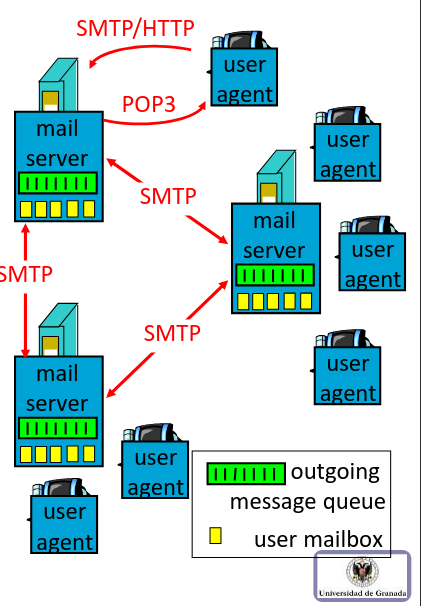
\includegraphics[width=0.5\textwidth]{images/correo.png}
    \caption{Proceso de envío de correo}
    \label{fig:correo}
\end{figure}

La interacción entre el cliente SMTP y el servidor SMTP se realiza mediante comandos y respuestas, siendo los comandos texto ASCII y las respuestas códigos de estado con frases explicativas. Los mensajes deben estar codificados en ASCII de 7 bits, pero con la definición posterior de las extensiones MIME, también es posible enviar mensajes en ASCII de 8 bits y formatos enriquecidos.

\subsubsection{Protocolos de Descarga (o Lectura): POP3, IMAP, HTTP}
Para leer o descargar los correos electrónicos del servidor de correo, se utilizan diferentes protocolos, entre los cuales los más comunes son POP3, IMAP y HTTP.

\subsubsection{Pasos en el Envío/Recepción de Correo}
A continuación se describen los pasos básicos en el proceso de envío y recepción de un mensaje de correo electrónico:

\begin{enumerate}
    \item El usuario origen compone un mensaje mediante su Agente de Usuario (MUA) dirigido al usuario destino.
    \item El mensaje se envía utilizando SMTP (o HTTP) al servidor de correo (MTA) del usuario origen, donde se coloca en la cola de mensajes salientes.
    \item El cliente SMTP abre una conexión TCP con el servidor de correo (MTA) del usuario destino, obtenido a través del sistema DNS.
    \item El cliente SMTP envía el mensaje a través de la conexión TCP.
    \item El servidor de correo del usuario destino coloca el mensaje en el buzón (mailbox) del usuario destino.
    \item El usuario destino invoca su Agente de Usuario (MUA) para leer el mensaje, utilizando POP3, IMAP o HTTP\footnote{Para ver los códigos de respuesta y de petición, accede a las diapositivas 78 y 79 del tema 5}.
\end{enumerate}



\begin{figure}[H]
    \centering
    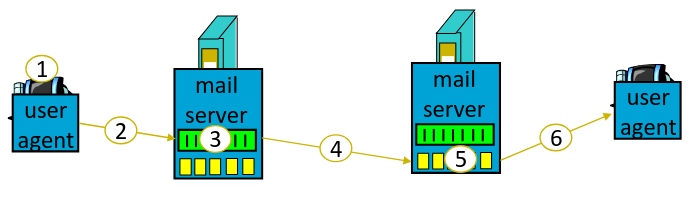
\includegraphics[width=0.7\textwidth]{images/pasos.png}
    \caption{Pasos en el envío y recepción de correo}
    \label{fig:pasos}
\end{figure}

\subsection{Multipurpose Internet Mail Extensions (MIME)}

Las extensiones MIME (Multipurpose Internet Mail Extensions) no cambian la arquitectura de correo electrónico, pero permiten soportar diversas funcionalidades adicionales. Los objetivos de MIME son:

\begin{itemize}
    \item Soportar texto en conjuntos de caracteres distintos de US-ASCII.
    \item Permitir adjuntos que no sean de tipo texto.
    \item Manejar cuerpos de mensajes con múltiples partes (multi-part).
    \item Incluir información de encabezados con conjuntos de caracteres distintos de ASCII.
\end{itemize}

MIME está especificado en seis RFCs: RFC 2045, RFC 2046, RFC 2047, RFC 4288, RFC 4289 y RFC 2077.

\subsubsection{No confundir los mensajes del protocolo con el formato de almacenamiento}
Es importante destacar que los mensajes MIME no deben confundirse con el formato de almacenamiento. Los mensajes MIME definen cómo los datos son representados para su transmisión a través de la red, mientras que el formato de almacenamiento puede diferir.

\subsubsection{Cabeceras de mensajes MIME}
Las cabeceras MIME permiten definir y gestionar diferentes aspectos de los mensajes. Algunas de las cabeceras más importantes son:

\begin{itemize}
    \item \textbf{MIME-Version}: Identifica la versión de MIME. Si no existe, se considera que el mensaje es texto normal en inglés.
    \item \textbf{Content-Description}: Cadena de texto que describe el contenido del mensaje, necesaria para que el destinatario sepa si desea descodificar y leer el mensaje.
    \item \textbf{Content-Id}: Identificador único, utiliza el mismo formato que la cabecera estándar \texttt{Message-Id}.
    \item \textbf{Content-Transfer-Encoding}: Indica la manera en que el cuerpo del mensaje está envuelto para su transmisión.
    \item \textbf{Content-Type}: Especifica la naturaleza del cuerpo del mensaje.
\end{itemize}

\subsubsection{Content-Transfer-Encoding}
Este campo indica cómo está envuelto el cuerpo del mensaje para su transmisión, ya que caracteres distintos de letras, números y signos de puntuación pueden generar problemas. Existen 5 tipos de codificación, especificados en la RFC 1521:

\begin{itemize}
    \item ASCII 7
    \item ASCII 8
    \item Codificación binaria
    \item Base64
    \item Codificación entrecomillada-imprimible
\end{itemize}

\subsubsection{Content-Type: Tipos y Subtipos}
El campo \texttt{Content-Type} define el tipo y subtipo del contenido del mensaje. La lista inicial de tipos y subtipos especificada por el RFC 1521 es la siguiente:

\begin{itemize}
    \item \textbf{Text/Plain}: Texto sin formato.
    \item \textbf{Text/Richtext}: Texto con comandos de formato sencillos.
    \item \textbf{Image/Gif}: Imagen fija en formato GIF.
    \item \textbf{Image/Jpeg}: Imagen fija en formato JPEG.
    \item \textbf{Audio/Basic}: Sonido.
    \item \textbf{Video/Mpeg}: Película en formato MPEG.
    \item \textbf{Application/Octet-stream}: Secuencia de bytes no interpretada.
    \item \textbf{Postscript}: Documento imprimible en formato PostScript.
    \item \textbf{Message/Rfc822}: Mensaje MIME en formato RFC 822.
    \item \textbf{Multipart/Mixed}: Partes independientes en el orden especificado.
    \item \textbf{Multipart/Alternative}: El mismo mensaje en diferentes formatos.
    \item \textbf{Multipart/Parallel}: Las partes deben verse simultáneamente.
    \item \textbf{Multipart/Digest}: Cada parte es un mensaje RFC 822 completo.
\end{itemize}

\subsubsection{Content-Type: Tipo \texttt{application}}
El tipo \texttt{application} es un tipo general para los formatos que requieren procesamiento externo no cubierto por otros tipos. El subtipo \texttt{octet-stream} es una secuencia de bytes no interpretada, y su recepción sugiere al usuario que lo copie en un archivo.

\subsubsection{Content-Type: Tipo \texttt{message}}
El tipo \texttt{message} permite que un mensaje esté completamente encapsulado dentro de otro. Los subtipos más comunes son:

\begin{itemize}
    \item \textbf{rfc822}: Se utiliza cuando un mensaje RFC 822 completo está encapsulado en un mensaje exterior.
    \item \textbf{partial}: Divide un mensaje en partes y las envía por separado. Los parámetros permiten ensamblar correctamente todas las partes.
    \item \textbf{external-body}: Usado para mensajes grandes (por ejemplo, archivos de vídeo), donde se proporciona una dirección FTP en lugar de incluir el archivo en el mensaje.
\end{itemize}

\subsubsection{Content-Type: Tipo \texttt{multipart}}
El tipo \texttt{multipart} permite que un mensaje contenga más de una parte. Los subtipos más comunes son:

\begin{itemize}
    \item \textbf{mixed}: Permite que cada parte sea diferente.
    \item \textbf{alternative}: Contiene el mismo mensaje en diferentes formatos.
    \item \textbf{parallel}: Las partes deben ser vistas simultáneamente, como en el caso de los canales de audio y vídeo de las películas.
    \item \textbf{digest}: Agrupa varios mensajes en un único mensaje compuesto\footnote{Ejemplo en la diapositiva 87 del tema 5}.
\end{itemize}

\subsection{Protocolo POP3 e IMAP4}

\subsubsection{Protocolo POP3}

El \textbf{Post Office Protocol 3} (POP3) es un protocolo utilizado para la descarga de correos electrónicos desde un servidor a un cliente. El puerto TCP utilizado por POP3 es el \texttt{110}. Este protocolo se organiza en tres fases: 

\begin{itemize}
    \item \textbf{Fase de Autorización}: En esta fase el cliente debe autenticarse en el servidor utilizando los comandos \texttt{USER} y \texttt{PASS}.
    \item \textbf{Fase de Transacción}: Durante esta fase el cliente puede interactuar con el servidor para listar mensajes (\texttt{LIST}), obtener mensajes específicos (\texttt{RETR}) o eliminar mensajes (\texttt{DELE}).
    \item \textbf{Fase de Actualización del Servidor}: Al finalizar la sesión, el servidor elimina los mensajes marcados para su eliminación y cierra la conexión.
\end{itemize}

\subsubsection{Comandos POP3}

\begin{itemize}
    \item \textbf{USER}: Permite la identificación del usuario, seguido del nombre de usuario que identifica al cliente en el servidor.
    \item \textbf{PASS}: Especifica la contraseña para el usuario previamente indicado con el comando \texttt{USER}.
    \item \textbf{STAT}: Proporciona información acerca de los mensajes en el servidor.
    \item \textbf{RETR}: Solicita la descarga de un mensaje especificado por su número.
    \item \textbf{DELE}: Elimina el mensaje especificado por su número.
    \item \textbf{LIST}: Lista los mensajes por su número.
    \item \textbf{NOOP}: Mantiene la conexión abierta en caso de inactividad.
    \item \textbf{TOP}: Muestra las primeras \texttt{n} líneas del mensaje, proporcionando los encabezados y una parte del cuerpo.
    \item \textbf{UIDL}: Solicita al servidor que envíe un identificador único para el mensaje especificado.
    \item \textbf{QUIT}: Finaliza la sesión, eliminando los mensajes marcados como eliminados y enviando el estado de la acción.
\end{itemize}

\subsubsection{Protocolo IMAP4}

El \textbf{Internet Message Access Protocol} versión 4 (IMAP4)\footnote{Más explicaciones y ejemplos de IMAP4 en las diapositivas 91, 92, 93 del tema 5.} permite trabajar con el correo electrónico de manera similar a si fuera local, manteniendo la organización en el servidor (MTA). Los estados de IMAP4 incluyen:

\begin{itemize}
    \item \textbf{No Autenticado (NA)}: El cliente aún no se ha autenticado.
    \item \textbf{Autenticado (A)}: El cliente ha iniciado sesión con éxito.
    \item \textbf{Seleccionado (S)}: El cliente ha seleccionado una carpeta o un mensaje específico.
    \item \textbf{Desconexión (D)}: El cliente ha cerrado la sesión.
\end{itemize}

\subsubsection{Comandos IMAP4}

IMAP4 utiliza una serie de comandos según el estado del cliente:

\begin{itemize}
    \item \textbf{CAPABILITY}: Obtiene la lista de capacidades del servidor IMAP.
    \item \textbf{LOGIN / AUTHENTICATE}: Permite la autenticación del usuario.
    \item \textbf{SELECT}: Selecciona una carpeta para acceder a los mensajes.
    \item \textbf{CREATE / DELETE}: Crea o elimina una carpeta.
    \item \textbf{LIST}: Lista las carpetas disponibles en el servidor.
    \item \textbf{APPEND}: Añade un mensaje a una carpeta.
    \item \textbf{FETCH}: Recupera un mensaje.
    \item \textbf{STORE}: Modifica los flags o atributos de un mensaje.
    \item \textbf{SEARCH}: Permite buscar mensajes con ciertos criterios.
\end{itemize}

\subsubsection{Ventajas de IMAP4}

IMAP4 ofrece varias ventajas sobre otros protocolos, como POP3:

\begin{itemize}
    \item \textbf{Organización en carpetas en el servidor}: IMAP permite que los correos se gestionen y organicen directamente en el servidor, lo que facilita su acceso desde distintos dispositivos.
    \item \textbf{Mantiene información entre sesiones}: Los flags y la organización de los mensajes se mantienen entre sesiones, lo que permite acceder a la misma estructura desde cualquier cliente.
    \item \textbf{Descarga de partes del mensaje}: IMAP permite descargar solo una parte del mensaje (como los encabezados) para optimizar el ancho de banda.
    \item \textbf{Acceso desde varios clientes}: IMAP permite acceder al mismo correo desde diferentes dispositivos, sin necesidad de descargarlo primero, a diferencia de POP3.
\end{itemize}

\subsubsection{Ventajas de Webmail}

El acceso al correo a través de Webmail, utilizando un navegador web y protocolos como HTTP o HTTPS, tiene sus propias ventajas:

\begin{itemize}
    \item \textbf{Acceso desde cualquier dispositivo}: Webmail permite acceder al correo desde cualquier lugar con conexión a Internet.
    \item \textbf{Organización en el servidor}: La organización de los correos se mantiene en el servidor, accesible desde cualquier cliente con HTTP.
    \item \textbf{Seguridad}: El uso de HTTPS mejora la seguridad, cifrando las comunicaciones entre el cliente y el servidor.
\end{itemize}
\subsection{Listado de Puertos Relacionados con el Correo Electrónico}

Los protocolos utilizados para el envío y recepción de correos electrónicos operan en puertos específicos. A continuación se presenta un listado de los puertos más comunes asociados a estos protocolos:

\begin{itemize}
    \item \textbf{POP3}: Puerto \texttt{110} - Protocolo utilizado para la descarga de correos electrónicos desde el servidor.
    \item \textbf{IMAP}: Puerto \texttt{143} - Protocolo utilizado para acceder y gestionar correos electrónicos en el servidor.
    \item \textbf{SMTP}: Puerto \texttt{25} - Protocolo utilizado para el envío de correos electrónicos.
    \item \textbf{HTTP}: Puerto \texttt{80} - Protocolo utilizado para la navegación web, también utilizado en el acceso a Webmail.
    \item \textbf{Secure SMTP (SSMTP)}: Puerto \texttt{465} - Versión segura de SMTP utilizando SSL/TLS para cifrar las comunicaciones.
    \item \textbf{Secure IMAP (IMAP4-SSL)}: Puerto \texttt{585} - Versión segura de IMAP utilizando SSL/TLS.
    \item \textbf{IMAP4 over SSL (IMAPS)}: Puerto \texttt{993} - IMAP sobre SSL, utilizado para una comunicación segura entre cliente y servidor.
    \item \textbf{Secure POP3 (SSL-POP)}: Puerto \texttt{995} - Versión segura de POP3 utilizando SSL/TLS para cifrar las comunicaciones.
\end{itemize}

\section{Aplicaciones Multimedia}

\subsection{Conceptos de Calidad de Servicio (QoS) y Aplicaciones Multimedia}

\subsubsection{Tecnología de Convergencia}

La \textbf{IP} (Internet Protocol) se considera una "tecnología de convergencia" porque permite integrar diferentes tipos de servicios de comunicación, como voz, datos, y vídeo, sobre una misma infraestructura. Esto facilita la integración de redes y servicios, ofreciendo una solución eficiente y flexible para la transmisión de información.

\subsubsection{Calidad de Servicio (QoS)}

La \textbf{Calidad de Servicio} (QoS, por sus siglas en inglés) se refiere a la capacidad de una red para ofrecer el rendimiento requerido por una aplicación, garantizando ciertos parámetros de rendimiento, como el ancho de banda, la latencia, el jitter, y la pérdida de paquetes. 

En las redes IP tradicionales, se ofrece un servicio de \textbf{mejor esfuerzo} (\textit{Best Effort}), lo que significa que no se garantizan niveles específicos de QoS, ya que todos los datos compiten por los mismos recursos de red sin priorización. Sin embargo, para aplicaciones multimedia, que requieren una calidad constante y predecible, es fundamental implementar técnicas de QoS para garantizar un rendimiento adecuado.

\subsubsection{Aplicaciones Multimedia}

Las aplicaciones multimedia, como audio, vídeo, juegos y comunicaciones en tiempo real, tienen necesidades de rendimiento específicas. A continuación, se describen algunos tipos de aplicaciones multimedia y sus características:

\begin{itemize}
    \item \textbf{Flujo de audio y vídeo (streaming) almacenado}: Este tipo de flujo se refiere a la transmisión de contenido previamente grabado, como en plataformas de \textit{streaming} como \textit{YouTube}.
    \item \textbf{Flujo de audio y vídeo en vivo}: En este caso, el contenido se transmite en tiempo real, como en emisoras de radio o servicios de IPTV (Televisión por protocolo de Internet).
    \item \textbf{Audio y vídeo interactivo}: Las aplicaciones que permiten una comunicación interactiva, como \textit{Skype} para videollamadas, requieren un alto rendimiento en términos de latencia y jitter.
\end{itemize}

\subsubsection{Características Fundamentales de las Aplicaciones Multimedia}

Las aplicaciones multimedia tienen varias características fundamentales que requieren un manejo especial por parte de la red:

\begin{itemize}
    \item \textbf{Elevado ancho de banda}: Las aplicaciones multimedia, especialmente el vídeo de alta calidad, requieren un ancho de banda significativo para garantizar una transmisión fluida y sin interrupciones.
    \item \textbf{Tolerancia relativamente alta a la pérdida de datos}: Estas aplicaciones pueden tolerar pequeñas pérdidas de datos sin que la calidad se vea gravemente afectada, pero no pueden soportar pérdidas significativas.
    \item \textbf{Exigen delay (retardo) acotado}: La latencia debe ser baja, ya que los retrasos en la transmisión de audio o vídeo pueden causar problemas de sincronización y afectar la experiencia del usuario.
    \item \textbf{Exigen jitter (fluctuación del retardo) acotado}: Las fluctuaciones en la latencia (jitter) deben mantenerse dentro de límites aceptables para evitar problemas en la calidad de la experiencia multimedia.
    \item \textbf{Beneficio del multicast}: Las aplicaciones multimedia pueden beneficiarse del uso de multicast, donde se envía el contenido a múltiples destinos a la vez, optimizando el uso de la red y mejorando la eficiencia.
\end{itemize}

\subsubsection{¿Cómo es un Router con QoS?}

Un \textbf{router con QoS} es un dispositivo de red capaz de gestionar el tráfico de forma que las aplicaciones con requisitos de rendimiento específicos reciban un tratamiento preferencial. Los routers con QoS implementan diversas técnicas de control, como la priorización de paquetes, la asignación de ancho de banda y la gestión de la congestión, para asegurar que los flujos de datos más importantes, como los de las aplicaciones multimedia, no sufran interrupciones o deterioro de calidad.

Algunas de las funcionalidades que un router con QoS puede implementar incluyen:

\begin{itemize}
    \item \textbf{Priorización de tráfico}: Los paquetes de datos de aplicaciones multimedia pueden ser priorizados sobre otros tipos de tráfico menos sensibles a la latencia o pérdida de paquetes, como el correo electrónico o la navegación web.
    \item \textbf{Asignación de ancho de banda}: El router puede reservar un cierto ancho de banda para las aplicaciones que lo necesiten, asegurando que el rendimiento no se vea afectado durante picos de tráfico.
    \item \textbf{Control de la congestión}: El router puede usar algoritmos de gestión de tráfico, como el control de la cola, para evitar la sobrecarga de la red y asegurar una distribución equitativa de los recursos.
    \item \textbf{Garantía de calidad}: Para aplicaciones que requieren un rendimiento garantizado, el router puede establecer mecanismos para asegurar que se mantengan los niveles de QoS especificados.
\end{itemize}

\begin{figure}[H]
    \centering
    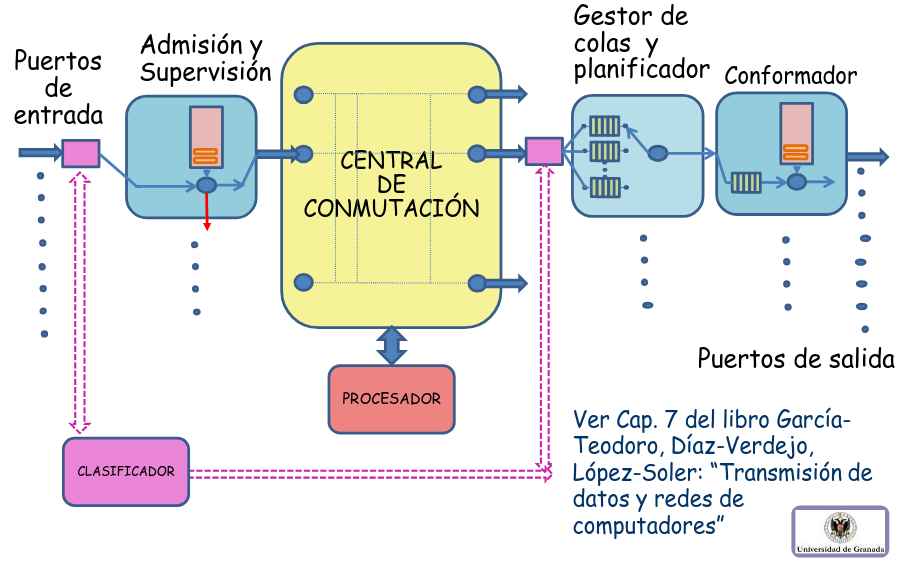
\includegraphics[width=0.7\textwidth]{images/QoS.png}
    \caption{Router con QoS}
    \label{fig:qos}
\end{figure}


\end{document}